\chapter{Resultados e Discussões} \label{cap:resultados}

Neste capítulo, são apresentados os resultados obtidos com a execução da metodologia proposta no \autoref{cap:desenvolvimento}, acompanhados da respectiva análise e discussão. A avaliação dos resultados é realizada com base nos cenários de ataques cibernéticos descritos na \autoref{sec:attacks}, com o objetivo de examinar a robustez das redes industriais OPC UA e a variação no desempenho dos componentes quando submetidos a esses cenários. Para melhor organização das informações, os resultados são estruturados em seções que correspondem a cada etapa da metodologia adotada.

De maneira geral, busca-se fornecer uma análise detalhada sobre as vulnerabilidades que podem ser exploradas durante o processo experimental. Caso essas hipóteses se confirmem, os achados deste estudo poderão contribuir para futuras melhorias no protocolo OPC UA e nos sistemas IACS, fortalecendo sua resiliência contra ameaças cibernéticas cada vez mais sofisticadas.

\section{Implementação da Bancada Experimental} \label{sec:impl-bancada}

    A \autoref{fig:banc} apresenta a bancada experimental utilizada para os ensaios de segurança cibernética, composta por um servidor OPC UA, um cliente OPC UA e um \textit{firewall} industrial. O servidor OPC UA tem a função de disponibilizar os dados de processo e gerenciar o sistema de automação industrial, enquanto o cliente OPC UA é responsável por acessar e visualizar essas informações. O \textit{firewall} industrial, por sua vez, desempenha um papel fundamental na supervisão e no controle do tráfego de dados entre o servidor e o cliente, garantindo a integridade e a segurança da comunicação na rede.

    \begin{figure}[htbp!]
        \caption{\label{fig:banc}Bancada experimental para ensaios de segurança cibernética}
        \begin{center}
            \includegraphics[width=0.5\textwidth]{USPSC-img/cyberkit2.png}
        \end{center}
        \legend{Fonte: elaborada pelo autor.}
    \end{figure}

\section{Aquisição dos Dados nos Cenários de Ataques Cibernéticos} \label{sec:exec-attacks}

    No estágio da metodologia descrito na \autoref{sec:aquisicao}, a bancada experimental é configurada de acordo com os cenários especificados (\autoref{tab:attacks}). Em seguida, o sistema de medição é acionado para realizar a captura do tráfego da rede e o monitoramento do desempenho do hospedeiro do servidor OPC UA, enquanto os ataques são executados. Para cada cenário, os dados de tráfego da rede OPC UA são coletados durante um período de 60 segundos.
    
    A \autoref{tab:carac-cenarios} apresenta um resumo detalhado das características do tráfego da rede e do desempenho do sistema em cada cenário de ataque, além da comunicação normal em redes OPC UA industriais.    

    \begin{table}[htbp!]
        \centering
        \caption{Informações do tráfego da rede e desempenho do hospedeiro em cada cenário}%
        \label{tab:carac-cenarios}
        \begin{tabular}{M{1.5cm}M{3cm}M{2.5cm}M{2.5cm}M{2cm}M{2cm}}
            \toprule
            \textbf{Cenário} & \textbf{\textit{Throughput} médio (kbits/s)} & \textbf{TP\textsuperscript{1} médio (Bytes)} & \textbf{PPS\textsuperscript{2} médio (pacotes/s)} & \textbf{Tráfego OPC UA (\%)} & \textbf{CPU\textsuperscript{3} (\%)} \\
            \toprule
            C1 & 130 & 127 & 128.4 & 28.7 & 7.31 \\
            \midrule
            C2 & 175 & 153 & 142.9 & 34.4 & 8.91 \\
            \midrule
            C3 & 179 & 162 & 138.3 & 31.8 & 9.01 \\
            \midrule
            C4 & 1166 & 965 & 151.1 & 9.2 & 17.16 \\
            \midrule
            C5 & 6824 & 972 & 877.9 & 5.3 & 10.64 \\
            \midrule
            C6 & 6894 & 973 & 885.9 & 8.2 & 10.78 \\
            \midrule
            C7 & 18000 & 60 & 38438.9 & 0.1 & 14.68 \\
            \midrule
            C8 & 12000 & 60 & 26788.9 & 0.1 & 13.23 \\
            \midrule
            C9 & 15000 & 60 & 31278.5 & 0.1 & 14.81 \\
            \midrule
            C10 & 462 & 171 & 337.3 & 72.9 & 9.86 \\
            \midrule
            C11 & 501 & 180 & 348.0 & 71.9 & 11.27 \\
            \midrule
            C12 & 491 & 184 & 334.1 & 69.8 & 11.36 \\
            \midrule
            C13 & 196 & 173 & 141.4 & 33.0 & 7.52 \\
            \midrule
            C14 & 235 & 195 & 151.3 & 35.2 & 9.03 \\
            \midrule
            C15 & 247 & 203 & 152.6 & 32.3 & 9.09 \\
            \midrule
            C16 & 105 & 125 & 105.3 & 33.1 & 6.80 \\
            \midrule
            C17 & 146 & 148 & 123.4 & 33.1 & 7.84 \\
            \midrule
            C18 & 137 & 159 & 107.9 & 33.2 & 7.96 \\
            \midrule
            C19 & 3410 & 43 & 10012.0 & 0.2 & 7.36 \\
            \midrule
            C20 & 3433 & 43 & 9896.4 & 0.2 & 7.97 \\
            \midrule
            C21 & 3432 & 44 & 9854.8 & 0.2 & 7.97 \\
            \midrule
            C22 & 168 & 127 & 166.1 & 32.1 & N/A \\
            \midrule
            C23 & 223 & 154 & 182.4 & 34.5 & N/A \\
            \midrule
            C24 & 219 & 162 & 169.7 & 32.5 & N/A \\
            \midrule
            C25 & 95 & 121 & 98.5 & 28.3 & 7.01 \\
            \midrule
            C26 & 253 & 142 & 222.7 & 17.9 & 7.95 \\
            \midrule
            C27 & 234 & 147 & 199.8 & 17.1 & 8.25 \\
            \bottomrule
            \multicolumn{6}{>{\tiny}l}{\textsuperscript{1} Tamanho do pacote.} \\
            \multicolumn{6}{>{\tiny}l}{\textsuperscript{2} Taxa de pacotes por segundo.} \\
            \multicolumn{6}{>{\tiny}l}{\textsuperscript{3} Processamento do hospedeiro do servidor OPC UA.} \\
        \end{tabular}
        \fonte{elaborada pelo autor.}%
    \end{table}

    O \textit{throughput} médio e o tamanho médio dos pacotes variam significativamente entre os cenários, refletindo a intensidade do tráfego gerado em cada situação. Os cenários de ataques de DoS por loop infinito na cadeia de certificados, como C1, C2 e C3, apresentam uma taxa de transferência de dados relativamente baixa. Em contraste, cenários como C7, C8 e C9, que envolvem DoS por inundação do TCP/IP, exibem um \textit{throughput} extremamente alto, evidenciando a intensa carga imposta à rede. Essa carga é particularmente perceptível pelo indicador crítico de intensidade do tráfego, PPS (taxa de pacotes por segundo), que atinge valores elevados nesses cenários.

    O percentual de tráfego OPC UA, embora varie drasticamente entre os cenários, não é, isoladamente, um fator determinante para a severidade do ataque. Por exemplo, cenários como C7, C8 e C9, que apresentam uma baixa porcentagem de tráfego OPC UA, ainda podem gerar uma carga substancial na rede devido ao alto PPS. Por outro lado, em cenários como C10, C11 e C12, onde a proporção de tráfego OPC UA é elevada, a alta taxa de pacotes por segundo pode não ser um fator predominante, mas indica que o ataque está direcionado especificamente aos protocolos de comunicação OPC UA.

    Além disso, o percentual de uso da CPU do controlador industrial (hospedeiro do servidor OPC UA) é um indicador relevante da sobrecarga imposta ao sistema durante os ataques. Cenários como C4, C5 e C6, que envolvem ataques de DoS por chamadas sucessivas de métodos OPC UA nulos, demonstram um aumento expressivo no consumo de processamento, sugerindo que esses ataques podem comprometer o desempenho do controlador, levando à degradação do serviço ou, em casos extremos, à sua interrupção.

    Essa análise ressalta a importância de considerar múltiplas métricas para avaliar o impacto dos diferentes tipos de ataques em redes OPC UA. Além da taxa de transferência de dados e da taxa de pacotes por segundo, fatores como o tamanho médio dos pacotes e a porcentagem de tráfego OPC UA são fundamentais para uma compreensão abrangente do comportamento da rede sob distintos cenários de ataque. A investigação detalhada dessas variáveis pode fornecer insights valiosos para o desenvolvimento de estratégias de mitigação e a implementação de medidas de segurança mais eficazes em ambientes industriais.

\section{Processamento dos Dados} \label{sec:processamento-dados}

    Após a coleta dos dados de tráfego da rede e do desempenho do hospedeiro do servidor OPC UA em cada cenário de ataque, o próximo passo consiste no processamento dessas informações para posterior análise e interpretação. Esse processamento é realizado pelo aplicativo \textbf{uanalyser}, cuja função é extrair dados relevantes a partir dos valores brutos e gerar métricas de desempenho específicas para cada situação.

    Na versão atual do aplicativo (v1.0.0), são gerados gráficos referentes a: (a) \textit{throughput} (kbps), (b) uso de recursos do hospedeiro do servidor OPC UA (RAM e CPU), (c) quantidade de pacotes OPC UA por segundo e (d) \textit{round trip time} (RTT) normalizado por pacote. A \autoref{fig:0-normal-local-server} apresenta um exemplo dos quatro gráficos de saída do aplicativo para o cenário C25.

    \begin{figure}[htbp!]
        \centering
        \caption{\label{fig:0-normal-local-server}Gráficos de condição normal de operação - nível de segurança: `None'.}
        \begin{subfigure}[t]{0.5\textwidth}
            \centering
            \caption{\textit{Throughput}}
            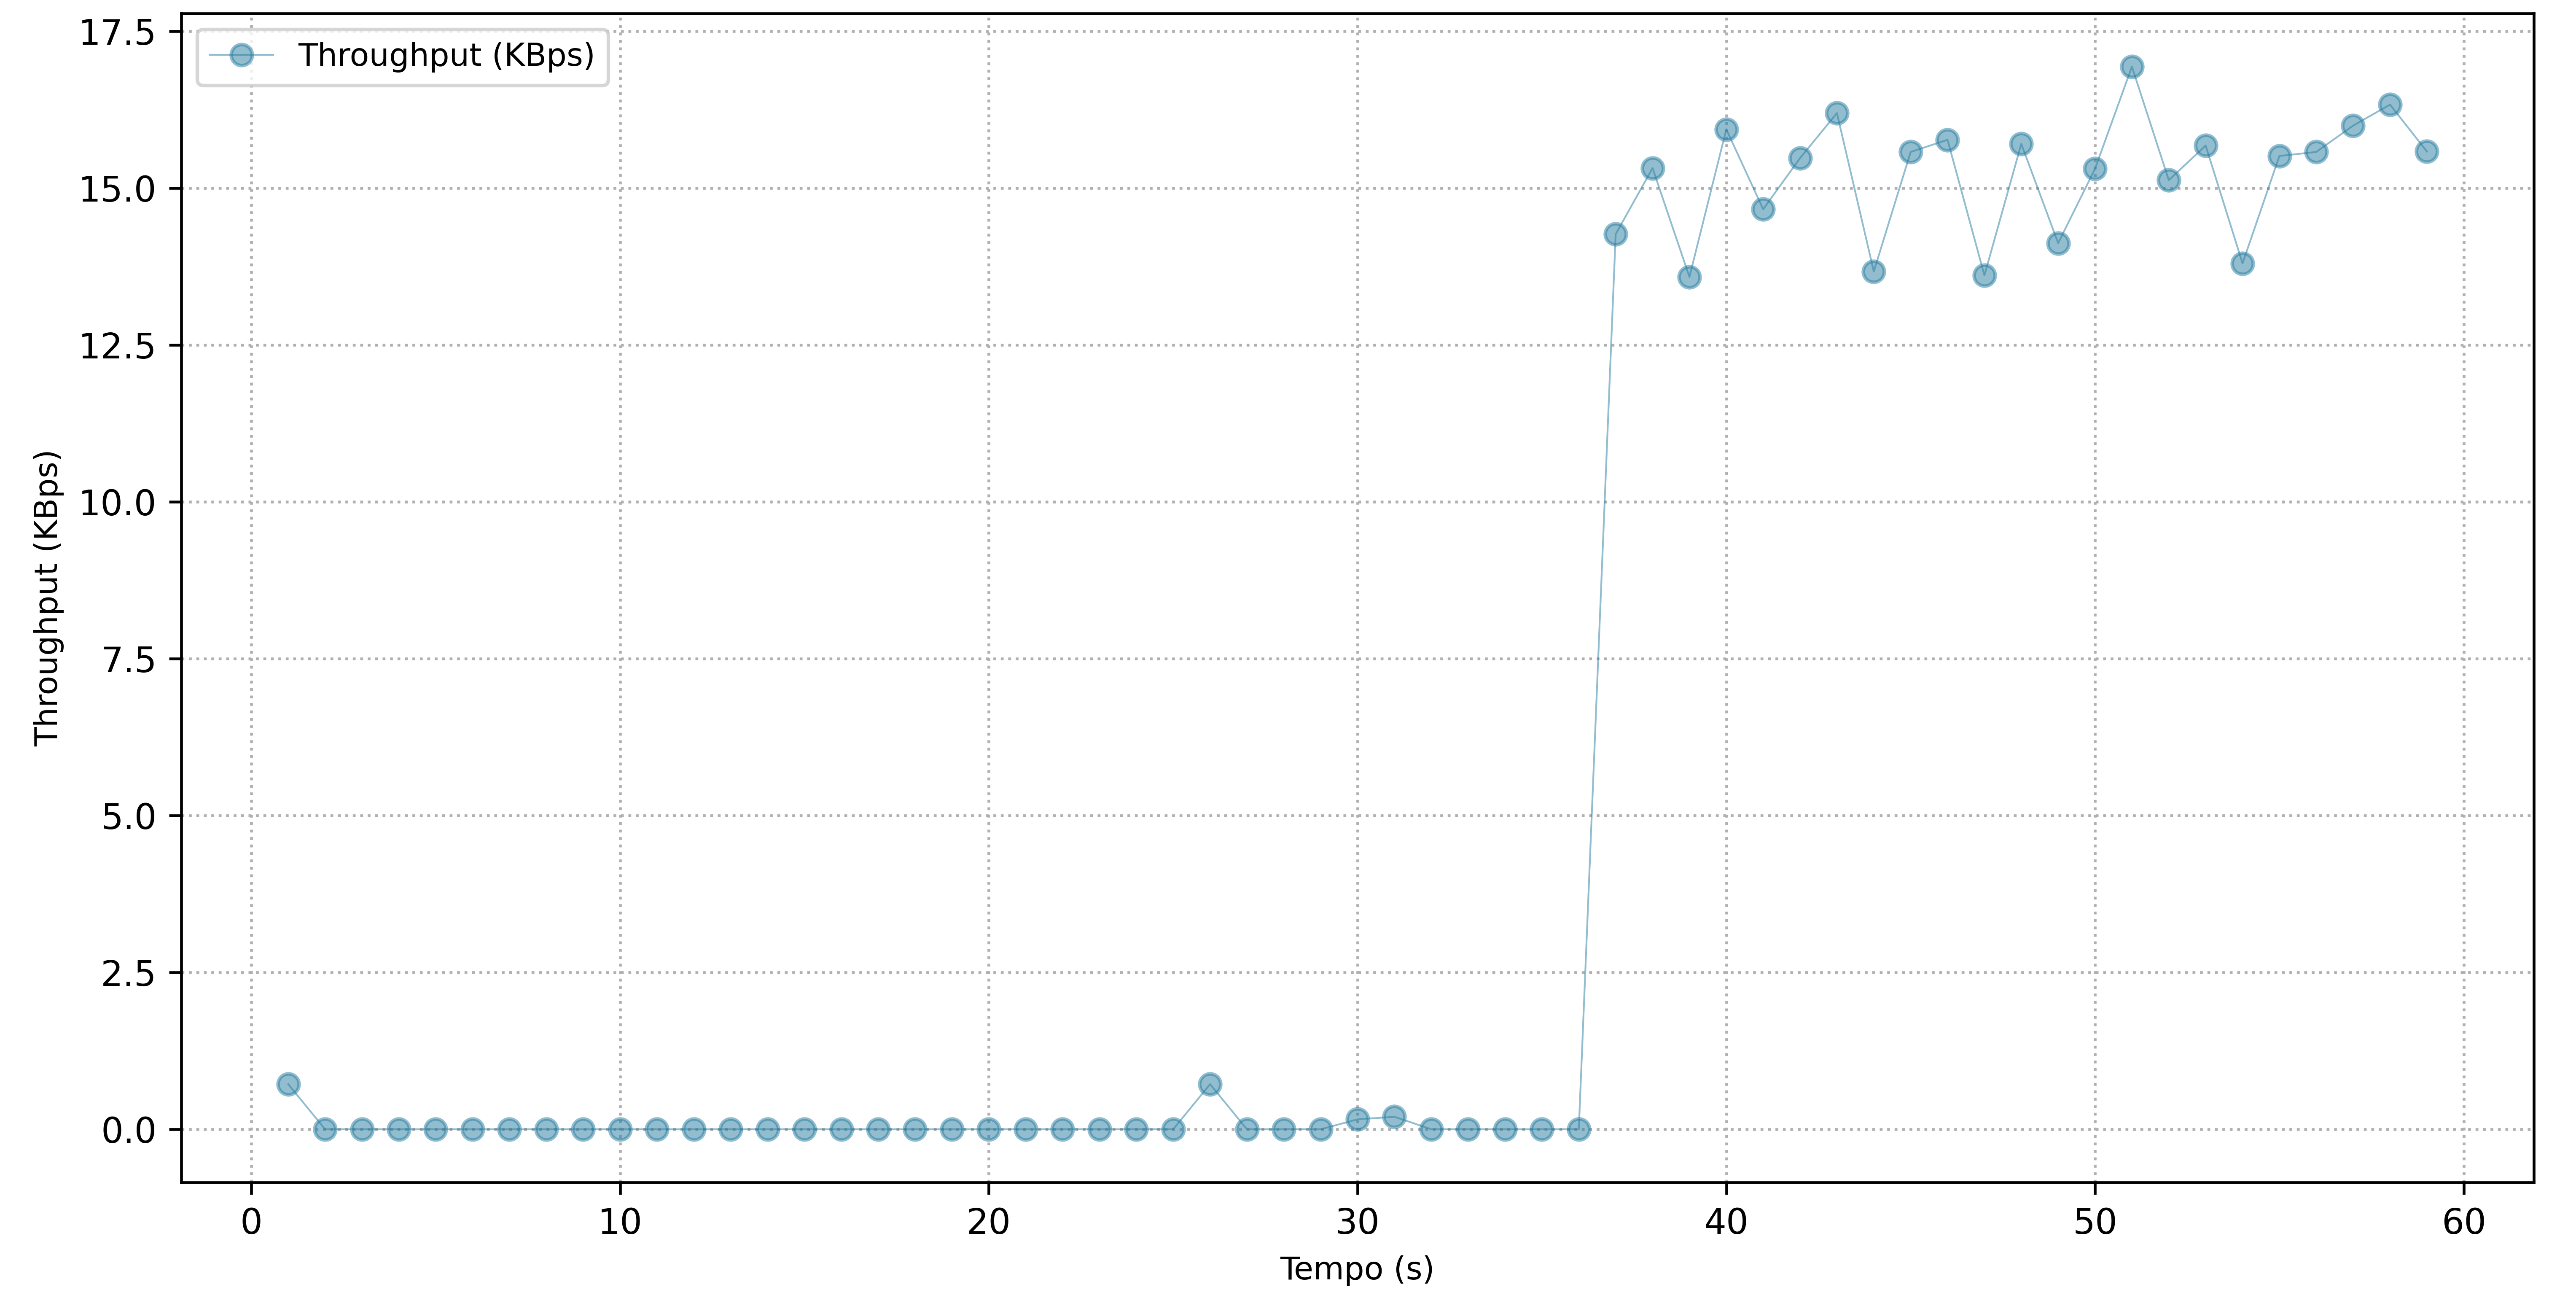
\includegraphics[width=1\textwidth, height=120pt]{USPSC-img/output/cropped/0-normal_local_server-tput.png}
        \end{subfigure}%
        ~ 
        \begin{subfigure}[t]{0.5\textwidth}
            \centering
            \caption{Desempenho}
            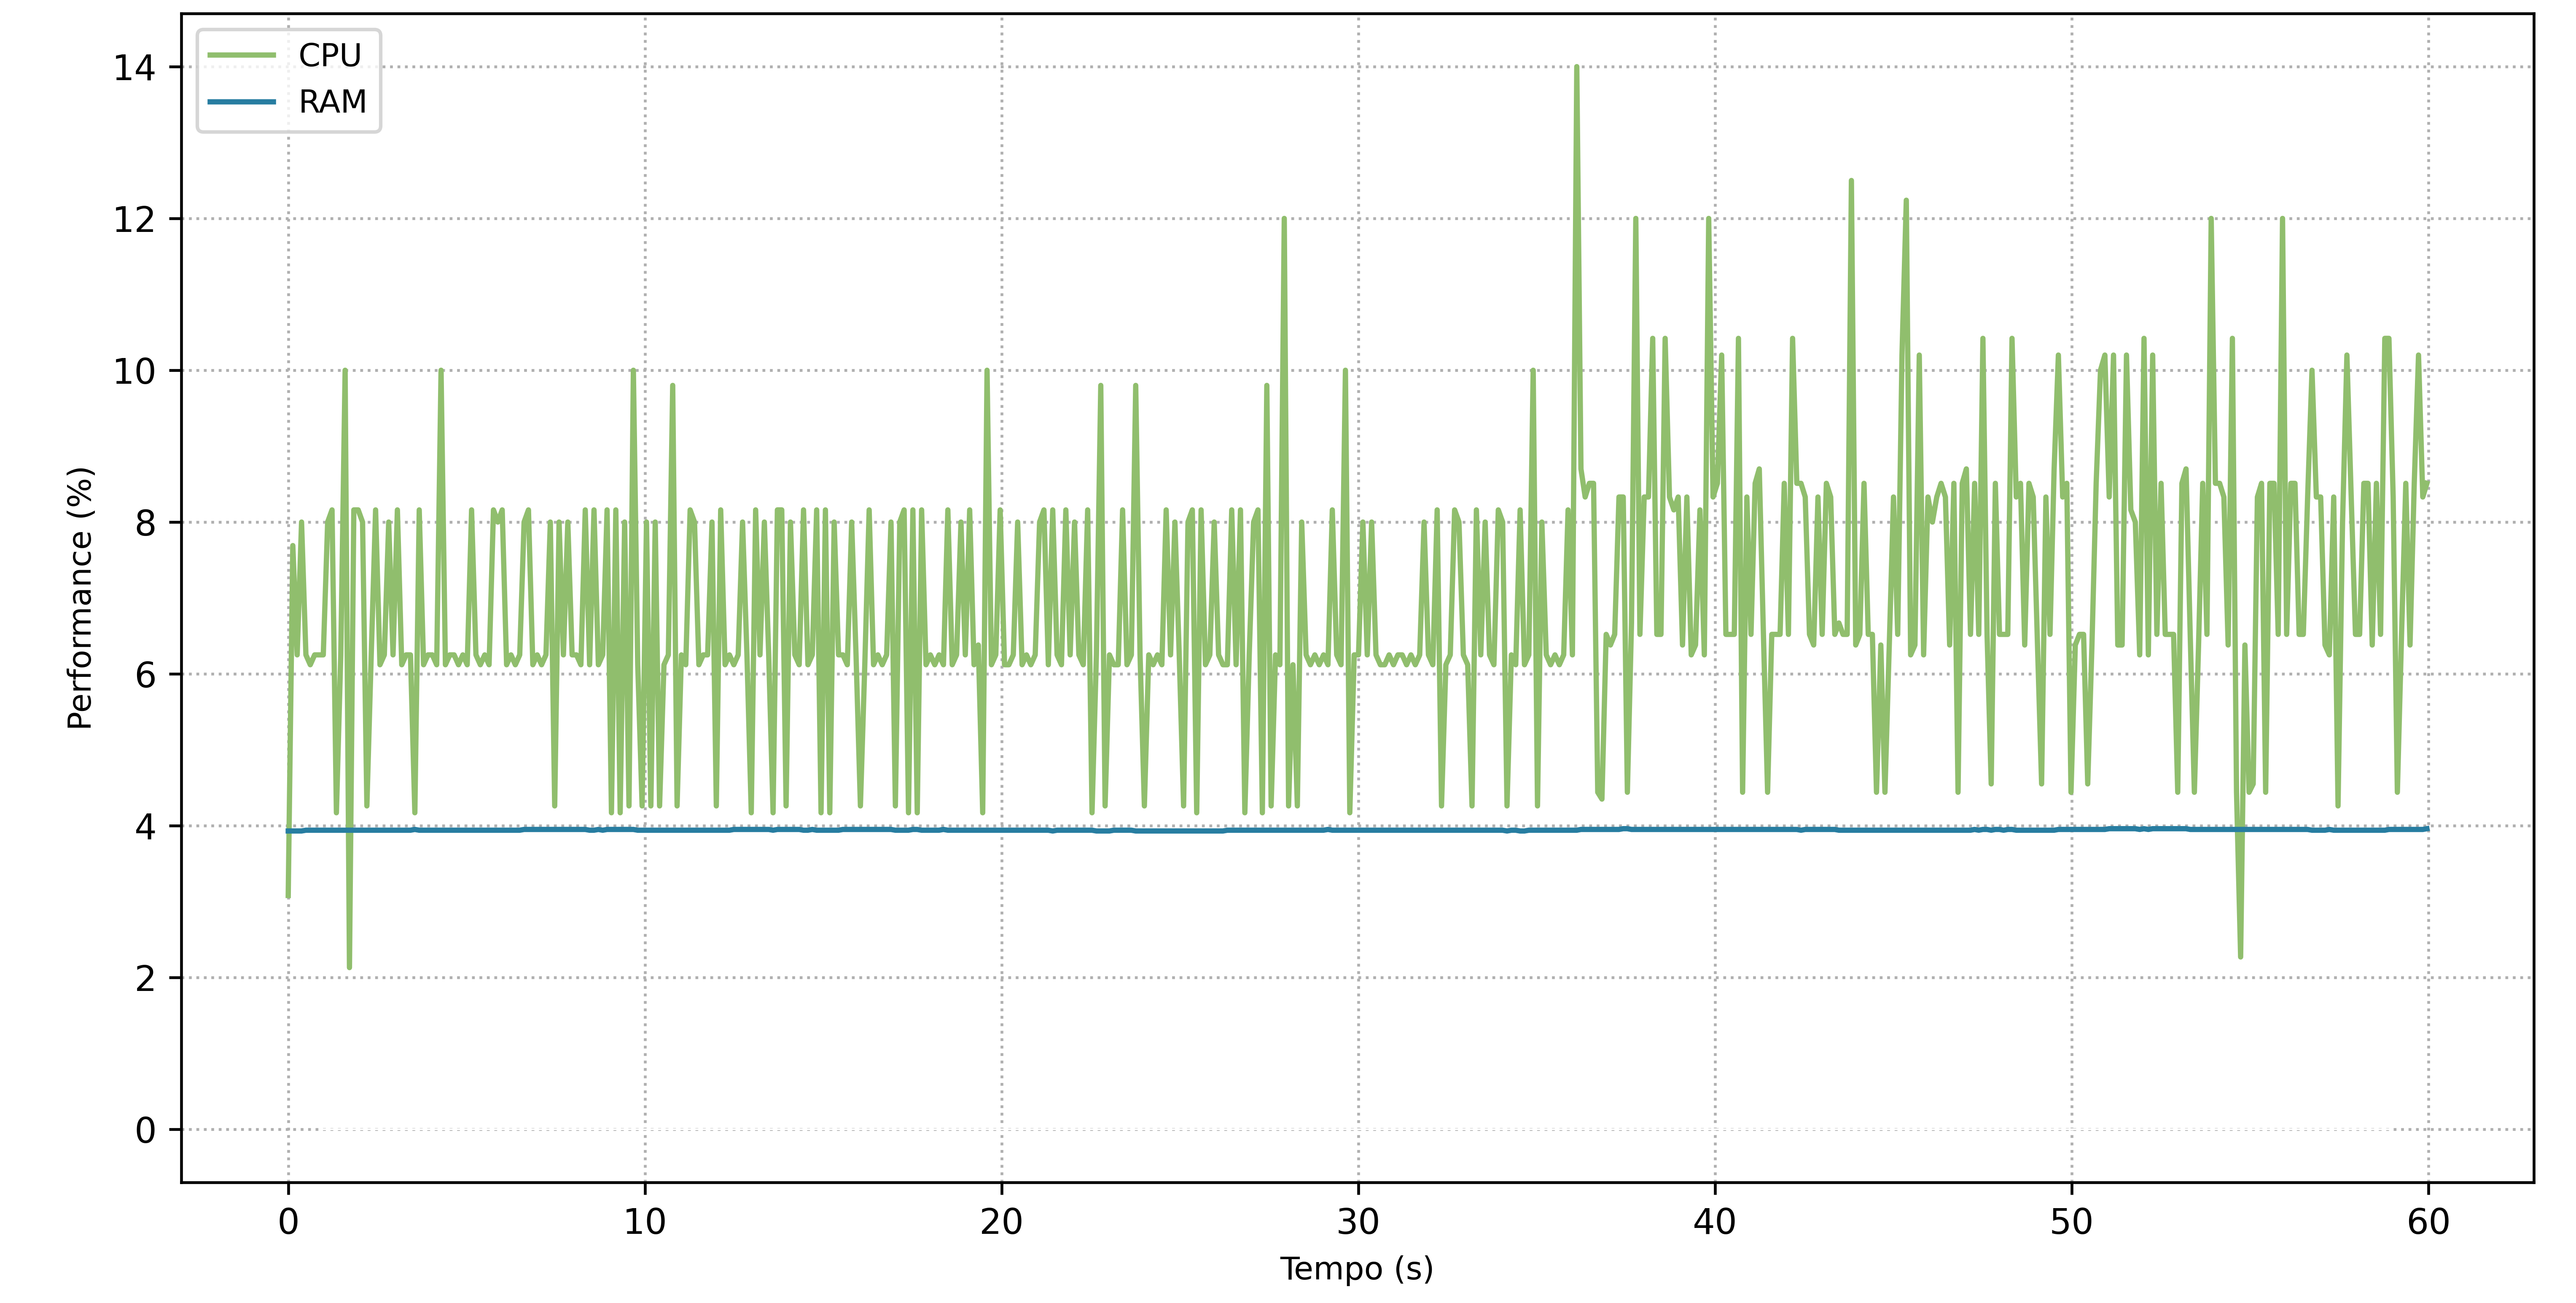
\includegraphics[width=1\textwidth, height=120pt]{USPSC-img/output/cropped/0-normal_local_server-perf.png}
        \end{subfigure}%
        \\
        \begin{subfigure}[t]{0.5\textwidth}
            \centering
            \caption{Pacotes OPC UA}
            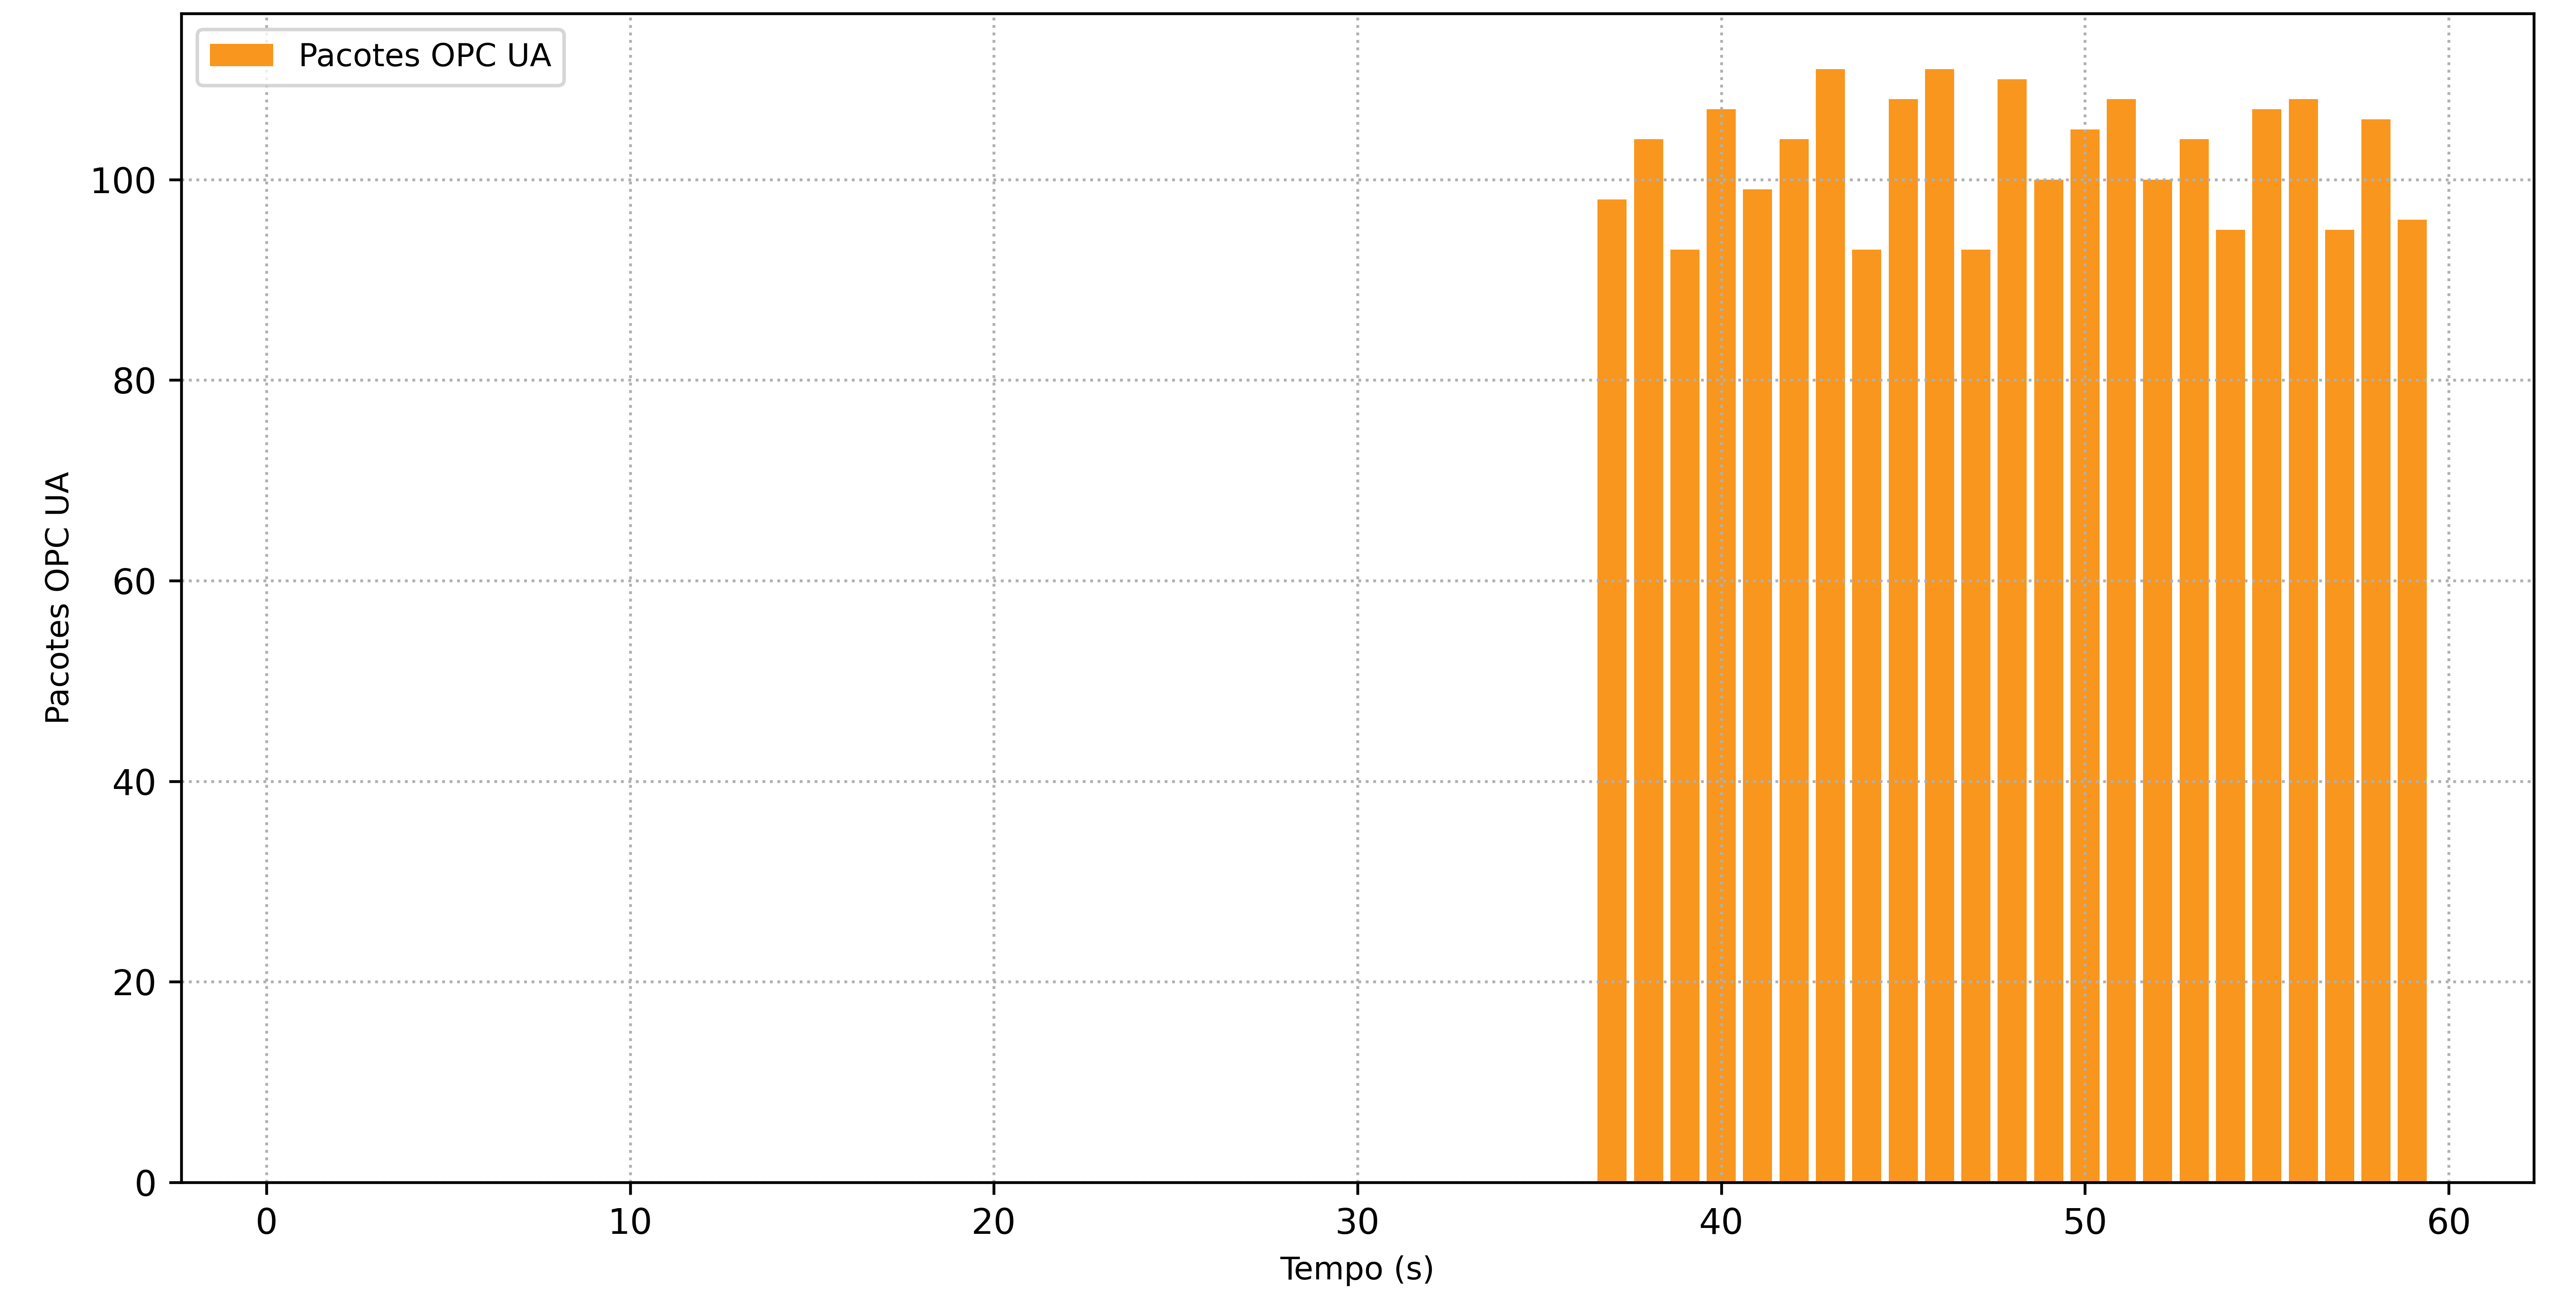
\includegraphics[width=1\textwidth, height=120pt]{USPSC-img/output/cropped/0-normal_local_server-pack.png}
        \end{subfigure}%
        ~
        \begin{subfigure}[t]{0.5\textwidth}
            \centering
            \caption{RTT por pacote}
            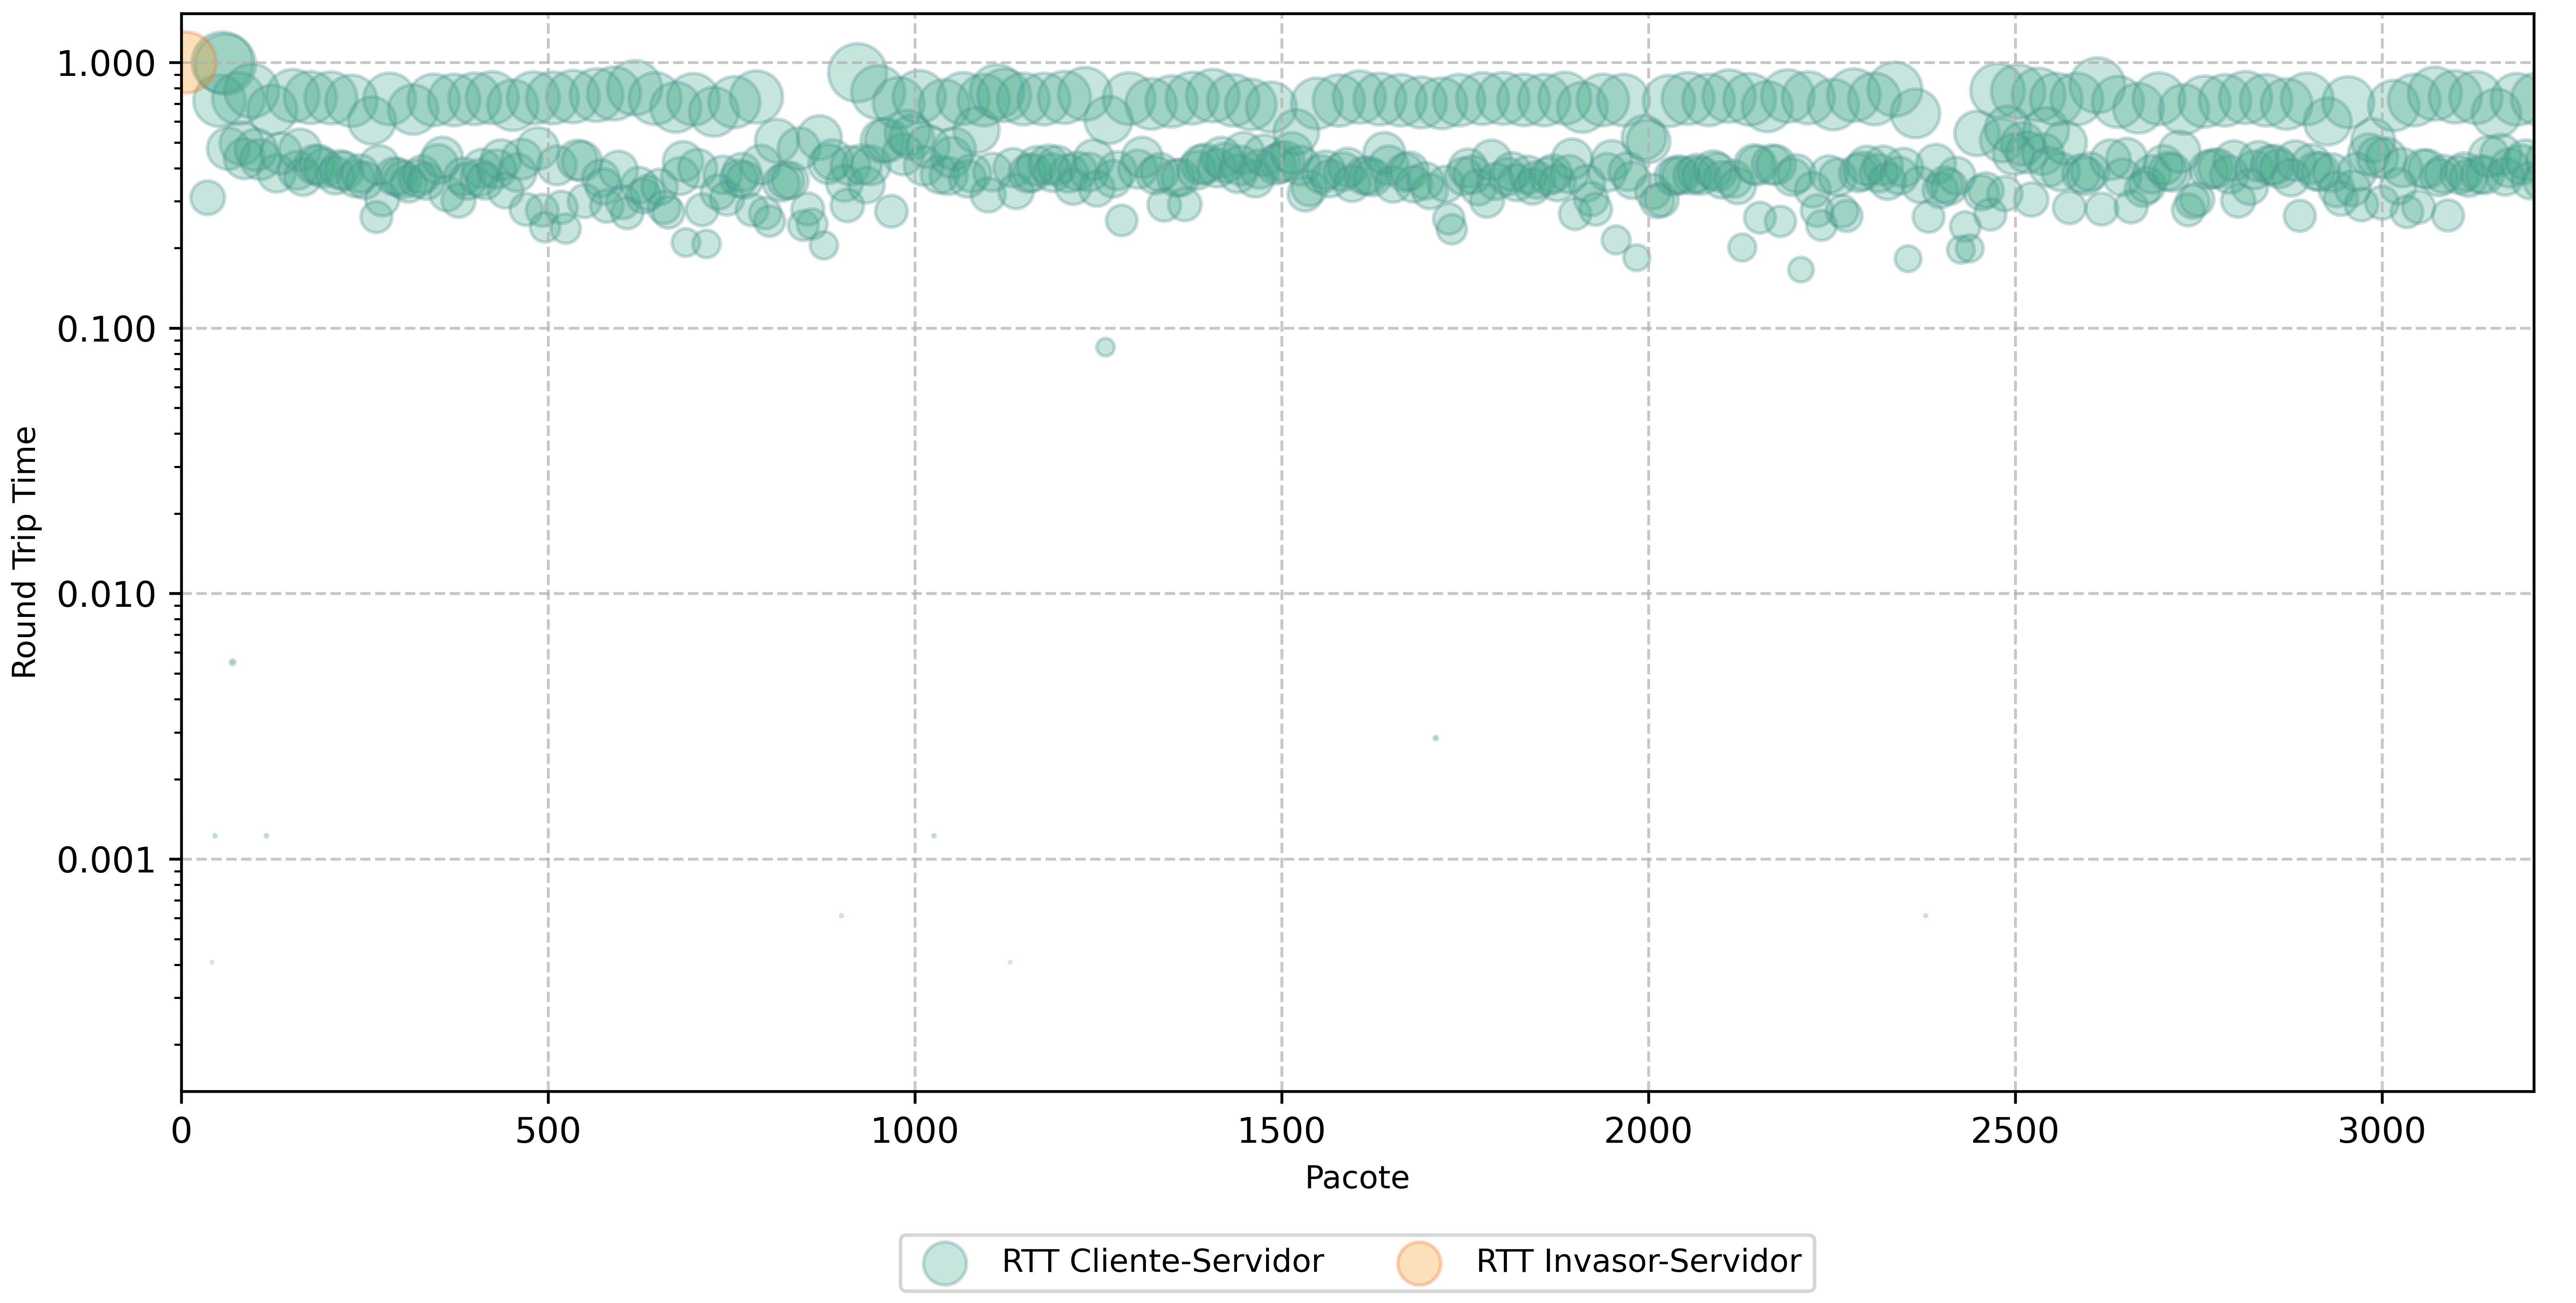
\includegraphics[width=1\textwidth, height=120pt]{USPSC-img/output/cropped/0-normal_local_server-rttp.png}
        \end{subfigure}%
        \legend{Fonte: elaborada pelo autor.}
    \end{figure}

    Os gráficos correspondentes aos demais cenários estão disponíveis no \autoref{ap:graficos}.

\section{Análise dos Resultados} \label{sec:analise-resultados}

    Nesta seção, são apresentadas as análises dos resultados obtidos a partir dos cenários de ataques cibernéticos executados na bancada experimental. A avaliação é realizada com base em métricas de desempenho extraídas dos dados coletados, com o objetivo de examinar a robustez das redes industriais OPC UA e as variações no desempenho dos componentes quando submetidos a tais ataques. Para melhor organização das informações, os resultados são segmentados em seções correspondentes a cada tipo de ataque.

    \subsection{\textit{Packet Sniffing}}

        Com o auxílio do Wireshark e do Ettercap, este primeiro ataque foi conduzido com o objetivo de identificar vulnerabilidades na rede OPC UA que possibilitem a interceptação não autorizada de pacotes. Inicialmente, o Ettercap foi empregado para a captura unificada de pacotes, enquanto o Wireshark foi utilizado para a análise detalhada do tráfego de rede. Durante a comunicação entre o servidor e o cliente, estabelece-se um canal seguro; contudo, um atacante pode explorar vulnerabilidades para interceptar pacotes e obter informações confidenciais, como os endereços IP e MAC de todos os dispositivos conectados. No início da captura para os cenários C22, C23 e C24, observam-se pacotes de comunicação entre o servidor e o cliente, conforme ilustrado na \autoref{fig:0-sniffing-wireshark}. Para facilitar a análise, aplicou-se um filtro que exibe exclusivamente os pacotes de comunicação OPC UA, omitindo demais dados na visualização. Todo o tráfego relevante relacionado ao protocolo OPC UA, representado na \autoref{fig:seqConn}, é analisado pelo Wireshark.

        \begin{figure}[htbp!]
            \caption{\label{fig:0-sniffing-wireshark}Comunicação interceptada entre o servidor e o cliente OPC UA com modo de segurança `None'}
            \begin{center}
                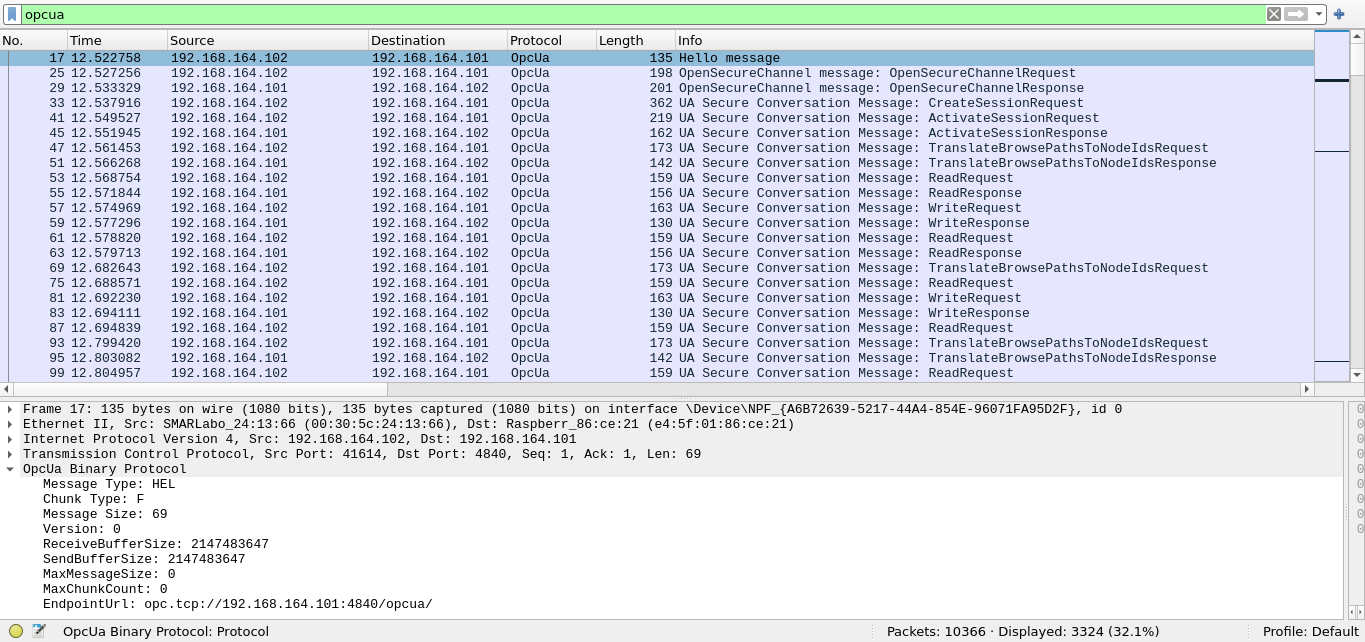
\includegraphics[width=0.972\textwidth]{USPSC-img/0-sniffing-wireshark-filtered-anon.png}
            \end{center}
            \legend{Fonte: elaborada pelo autor.}
        \end{figure}

        Vale ressaltar que o invasor possui o endereço IP 192.168.164.115 e está apenas conectado à rede, sem interação física com o servidor (192.168.164.101) ou com o cliente (192.168.164.102). Nos modos de segurança `None' e `Sign', a interceptação permite que o invasor obtenha todos os dados sensíveis trocados entre o servidor e o cliente, conforme ilustrado na \autoref{fig:writeRequest}, que representa a captura de um pacote de requisição de escrita (\textit{UA Secure Conversation Message: WriteRequest}) do mesmo valor e nó, enviado do cliente para o servidor.

        \begin{figure}[htbp!]
            \centering
            \caption{\label{fig:writeRequest}Informações obtidas pelo invasor com modo de segurança `None' e `Sign'}
            \begin{subfigure}[t]{0.5\textwidth}
                \centering
                \caption{`None'}
                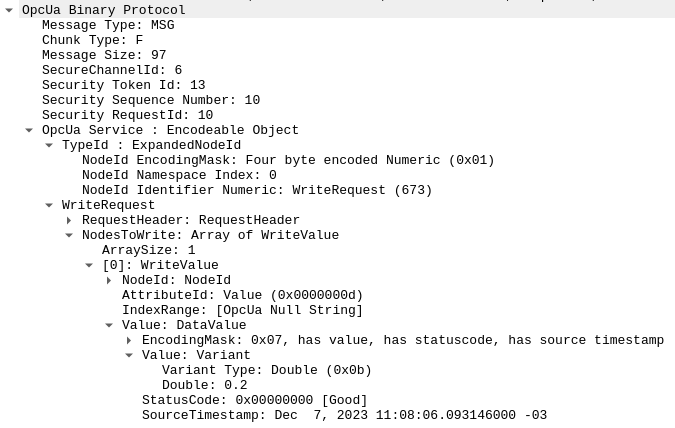
\includegraphics[width=1\textwidth]{USPSC-img/0-sniffing-WriteRequest.png}
            \end{subfigure}%
            ~ 
            \begin{subfigure}[t]{0.5\textwidth}
                \centering
                \caption{`Sign'}
                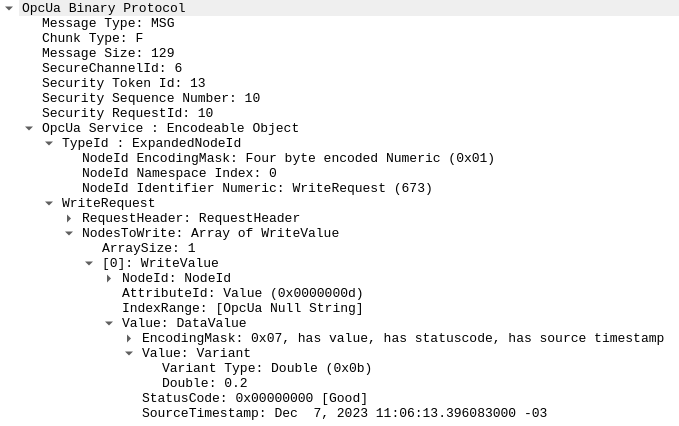
\includegraphics[width=1\textwidth]{USPSC-img/1-sniffing-WriteRequest.png}
            \end{subfigure}%
            \legend{Fonte: elaborada pelo autor.}
        \end{figure}

        Entretanto, ao configurar a comunicação no modo de segurança `Sign \& Encrypt', o invasor não consegue acessar informações sensíveis da troca de mensagens, pois os dados, além de assinados, são criptografados com políticas mais robustas, como a Basic256Sha256. Assim, no cenário C24, embora o tráfego continue sendo interceptado, a comunicação OPC UA não pode ser decifrada, uma vez que todos os pacotes do tipo MSG, identificados pela mensagem \textit{UA Secure Conversation Message: ServiceId [ID]}, apresentam o campo de dados \texttt{NodeId EncodingMask} como desconhecido.

        Dessa forma, este ataque demonstra o potencial comprometimento da segurança da rede OPC UA em cenários onde a comunicação é configurada com modos de segurança mais fracos, como `None' e `Sign'. Os resultados evidenciam que, utilizando ferramentas acessíveis e tendo acesso ao segmento principal da rede, um invasor pode facilmente realizar ataques de captura de pacotes, comprometendo a confidencialidade dos dados. Além disso, o atacante pode registrar todo o tráfego capturado e, posteriormente, utilizá-lo para outras ofensivas, como inserção de pacotes maliciosos (\textit{packet injection}), ataques de negação de serviço (DoS), ataques man-in-the-middle (MITM) e ataques distribuídos de negação de serviço (DDoS).

    \subsection{\textit{Man in the Middle (MITM)}}

        Após a execução bem-sucedida do ataque de \textit{Packet Sniffing}, o invasor passa a ter acesso a uma lista de endereços de todos os dispositivos da rede, além de informações sensíveis sobre o hospedeiro do servidor OPC UA, incluindo o \texttt{EndpointURI}. Com esses dados, torna-se viável a realização de um ataque do tipo MITM, permitindo não apenas a interceptação da comunicação, mas também o controle total sobre os dados transmitidos.

        Ambas as técnicas empregadas para a execução do ataque MITM foram realizadas com êxito. A abordagem baseada na falsificação da tabela ARP, aplicada nos cenários C16, C17 e C18, demonstrou que a comunicação pode ser interceptada e redirecionada para o invasor, possibilitando a captura e modificação dos pacotes de dados. A \autoref{fig:0-mitm-wireshark} ilustra a captura de pacotes de comunicação entre o servidor e o cliente, evidenciando o invasor atuando como intermediário. Ao comparar com o tráfego apresentado na \autoref{fig:0-sniffing-wireshark}, observa-se que o fluxo normal de comunicação é desviado para o invasor, identificado pelo endereço MAC \texttt{00:09:5B:A0:5F:F0}.

        \begin{figure}[htbp!]
            \centering
            \caption{\label{fig:0-mitm-wireshark}Interceptação de pacotes no ataque MITM com modo de segurança `None'}
            \begin{subfigure}[t]{1\textwidth}
                \centering
                \caption{\texttt{OpenSecureChannelRequest}}
                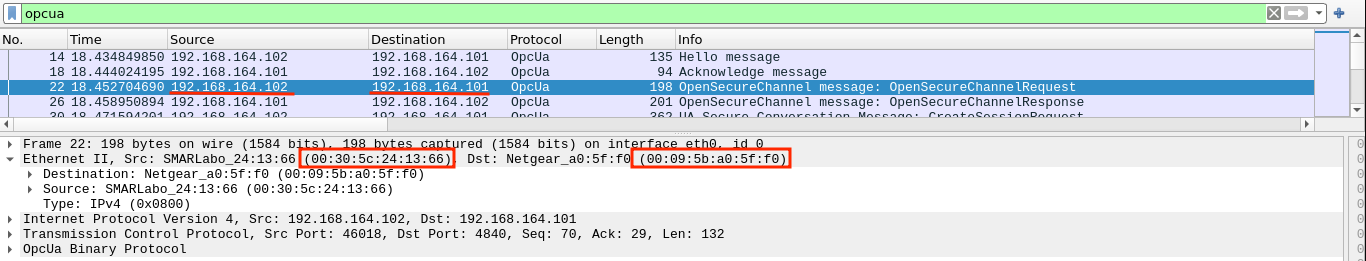
\includegraphics[width=1\textwidth]{USPSC-img/0-mitm-arp_1.png}
            \end{subfigure}%
            \\
            \begin{subfigure}[t]{1\textwidth}
                \centering
                \caption{\texttt{OpenSecureChannelResponse}}
                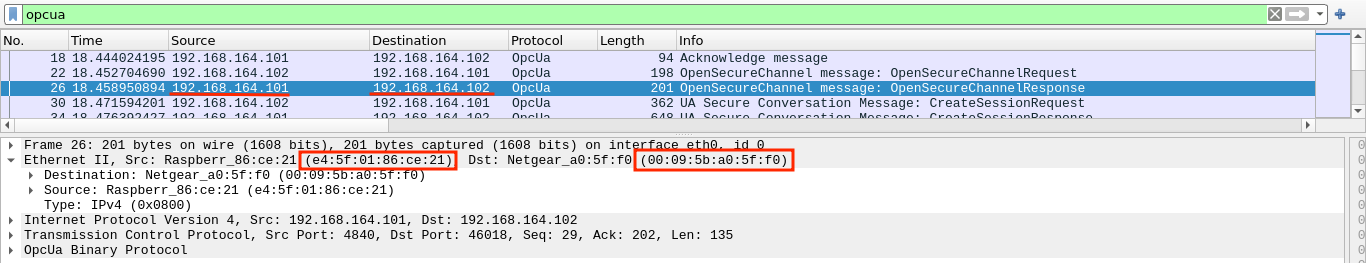
\includegraphics[width=1\textwidth]{USPSC-img/0-mitm-arp_2.png}
            \end{subfigure}%
            \legend{Fonte: elaborada pelo autor.}
        \end{figure}

        O processo inicia-se com a etapa de handshake entre os agentes, na qual o cliente estabelece a comunicação inicial e o servidor responde ao reconhecimento. Em seguida, o cliente envia uma solicitação \textit{OpenSecureChannelRequest}, à qual o servidor responde com uma \textit{OpenSecureChannelResponse}. Após essa fase, um \textit{SecureChannel} é estabelecido, seguido pelo envio da requisição \textit{CreateSessionRequest} pelo cliente e da respectiva resposta \textit{CreateSessionResponse} pelo servidor. Uma vez que a sessão é criada, ambos os agentes a ativam por meio das mensagens \textit{ActivateSessionRequest} e \textit{ActivateSessionResponse}. A partir desse ponto, quando o cliente acessa qualquer informação do servidor, são observadas as trocas de mensagens \textit{ReadRequest} e \textit{ReadResponse}.

        No ataque MITM baseado no roubo de portas, realizado nos cenários C19, C20 e C21, verificou-se um aumento expressivo no \texttt{throughput}, atingindo valores até dez vezes superiores aos registrados na técnica de falsificação da tabela ARP. Esse crescimento deve-se ao fato de que o ataque satura a tabela ARP do servidor por meio do envio massivo de pacotes ARP, forçando o redirecionamento do tráfego para o invasor. Em média, 99,3\% dos pacotes transmitidos nesses cenários são provenientes de \textit{broadcast} ARP. No entanto, mesmo quando essa abordagem é bem-sucedida e a interceptação é efetivada, observa-se que a comunicação não ocorre diretamente através do invasor, mas sim entre o servidor e o cliente, sendo redirecionada para a porta previamente comprometida.

        Com ambas as técnicas analisadas, verificou-se que algumas informações confidenciais podem ser acessadas pelo invasor, incluindo o \texttt{EndpointURI} do servidor, a \texttt{SecurityPolicy} e o \texttt{SecurityMode} utilizados na comunicação, bem como os dados coletados pelo servidor OPC UA em tempo real na rede do chão de fábrica. No entanto, ressalta-se que, quando a comunicação está configurada no nível de segurança mais elevado (`Sign \& Encrypt') e utiliza políticas de segurança atualizadas, o invasor não é capaz de decifrar os pacotes interceptados. Além disso, presume-se que, para a execução desse ataque, seja necessário acesso físico à rede, o que, em ambientes industriais, representa uma barreira significativa para potenciais invasores.

    \subsection{\textit{Denial of Service (DoS)}}

        Nesta seção, são apresentados os resultados obtidos a partir da execução de ataques de negação de serviço (DoS) na bancada experimental, empregando cinco técnicas distintas. O objetivo desses ataques é avaliar a resiliência da rede industrial OPC UA frente a sobrecargas de tráfego, além de analisar a variação no comportamento dos componentes quando submetidos a tais condições adversas.

        \subsubsection*{\underline{Inundação TCP/IP}}
    
            A execução do ataque por inundação TCP/IP (cenários C7, C8 e C9) teve início com uma varredura da rede para identificar dispositivos e serviços ativos, utilizando a ferramenta Nmap. Os resultados dessa análise revelaram a presença de um servidor OPC UA em funcionamento, com a respectiva porta aberta para comunicação. Com base nessas informações, a etapa seguinte consistiu na geração de uma inundação de pacotes SYN sobre a comunicação TCP/IP.
            
            Os resultados obtidos nesses cenários indicam uma alta vulnerabilidade da rede a ataques de inundação TCP/IP, evidenciada pelo aumento expressivo no \texttt{throughput} e na taxa de pacotes por segundo. O servidor OPC UA foi sobrecarregado devido à intensa carga de tráfego, resultando em um aumento substancial no uso da CPU e na consequente degradação do desempenho do sistema. O gráfico apresentado na \autoref{fig:perf-dos-tcp} ilustra a variação média no consumo de CPU do hospedeiro do servidor OPC UA durante a execução do ataque. Para facilitar a visualização e análise dos dados, foi empregada a técnica de média móvel, que suaviza a série temporal ao reduzir flutuações de curto prazo e destacar tendências de longo prazo.

            \begin{figure}[htbp!]
                \centering
                \caption{\label{fig:perf-dos-tcp}Variação média no processamento do hospedeiro do servidor OPC UA durante o ataque de inundação TCP/IP}
                \begin{subfigure}[t]{1\textwidth}
                    \centering
                    \caption{`None'}
                    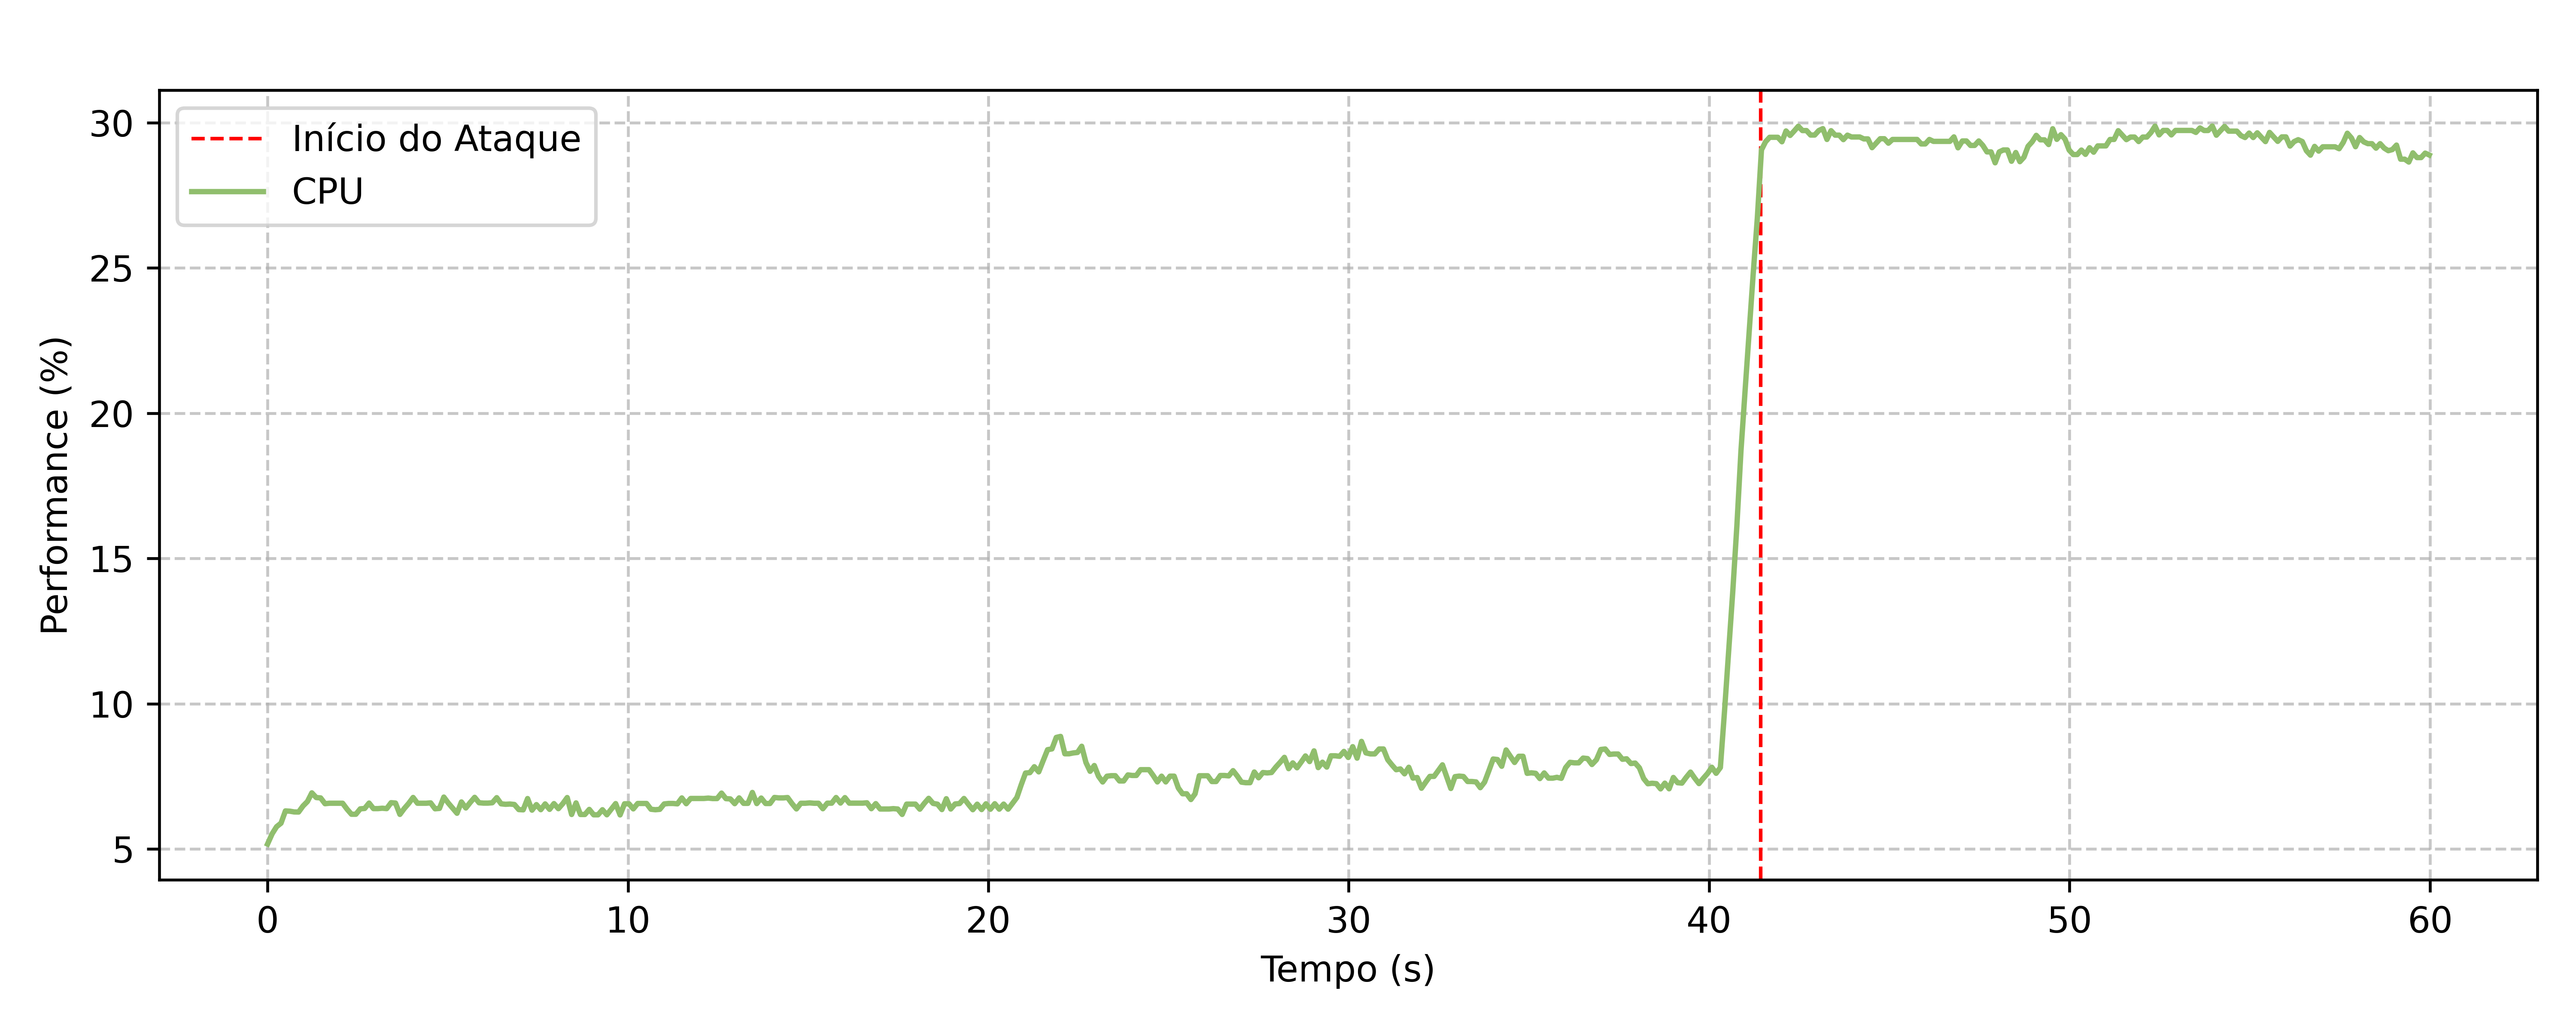
\includegraphics[width=1\textwidth]{USPSC-img/0-dos-hping-cpu.png}
                \end{subfigure}%
                \\
                \begin{subfigure}[t]{1\textwidth}
                    \centering
                    \caption{`Sign'}
                    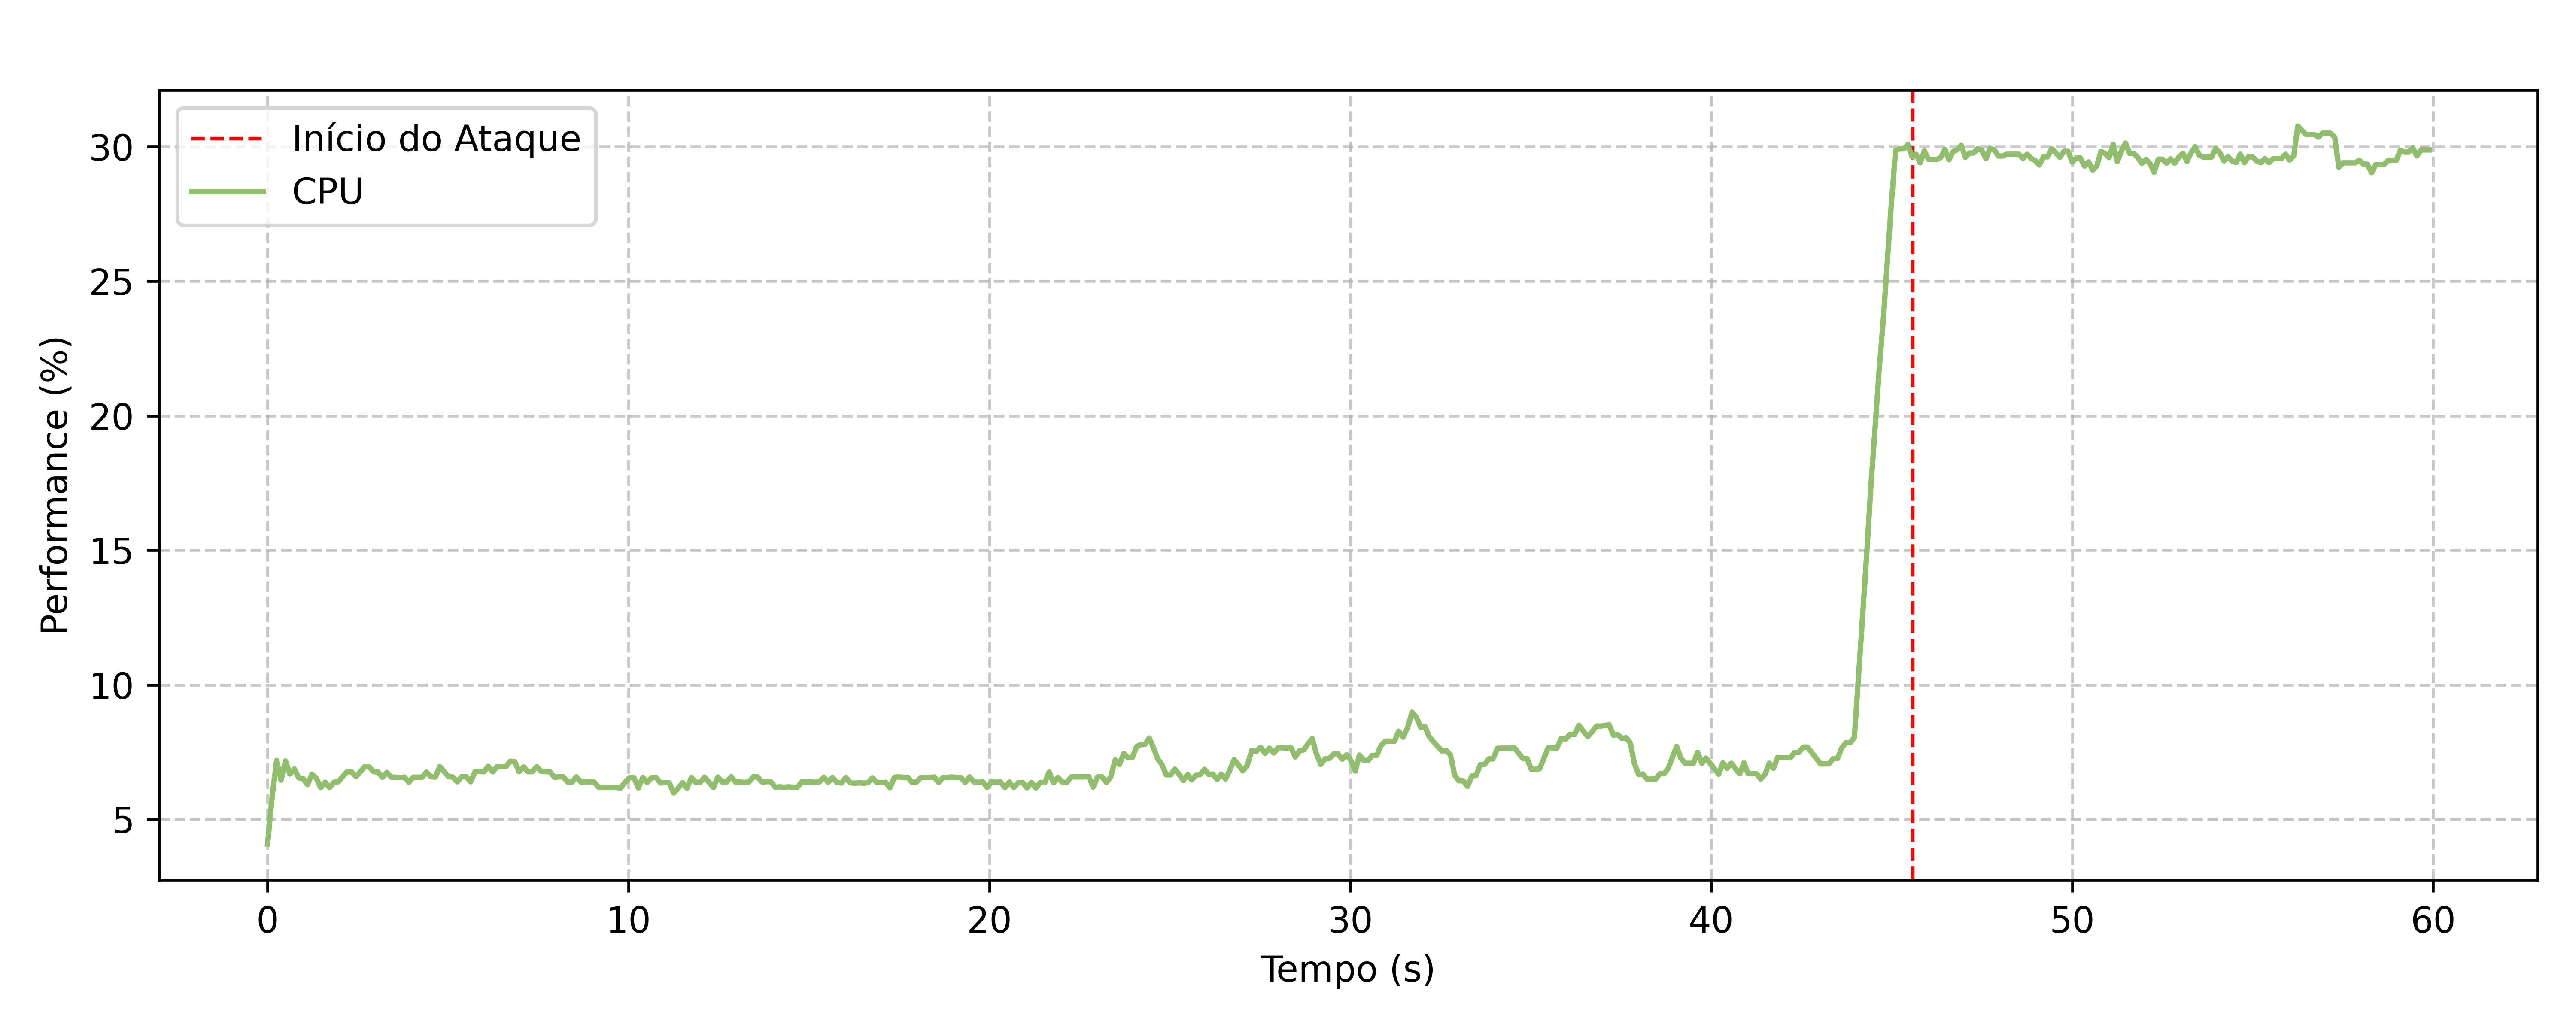
\includegraphics[width=1\textwidth]{USPSC-img/1-dos-hping-cpu.png}
                \end{subfigure}%
                \\
                \begin{subfigure}[t]{1\textwidth}
                    \centering
                    \caption{`Sign \& Encrypt'}
                    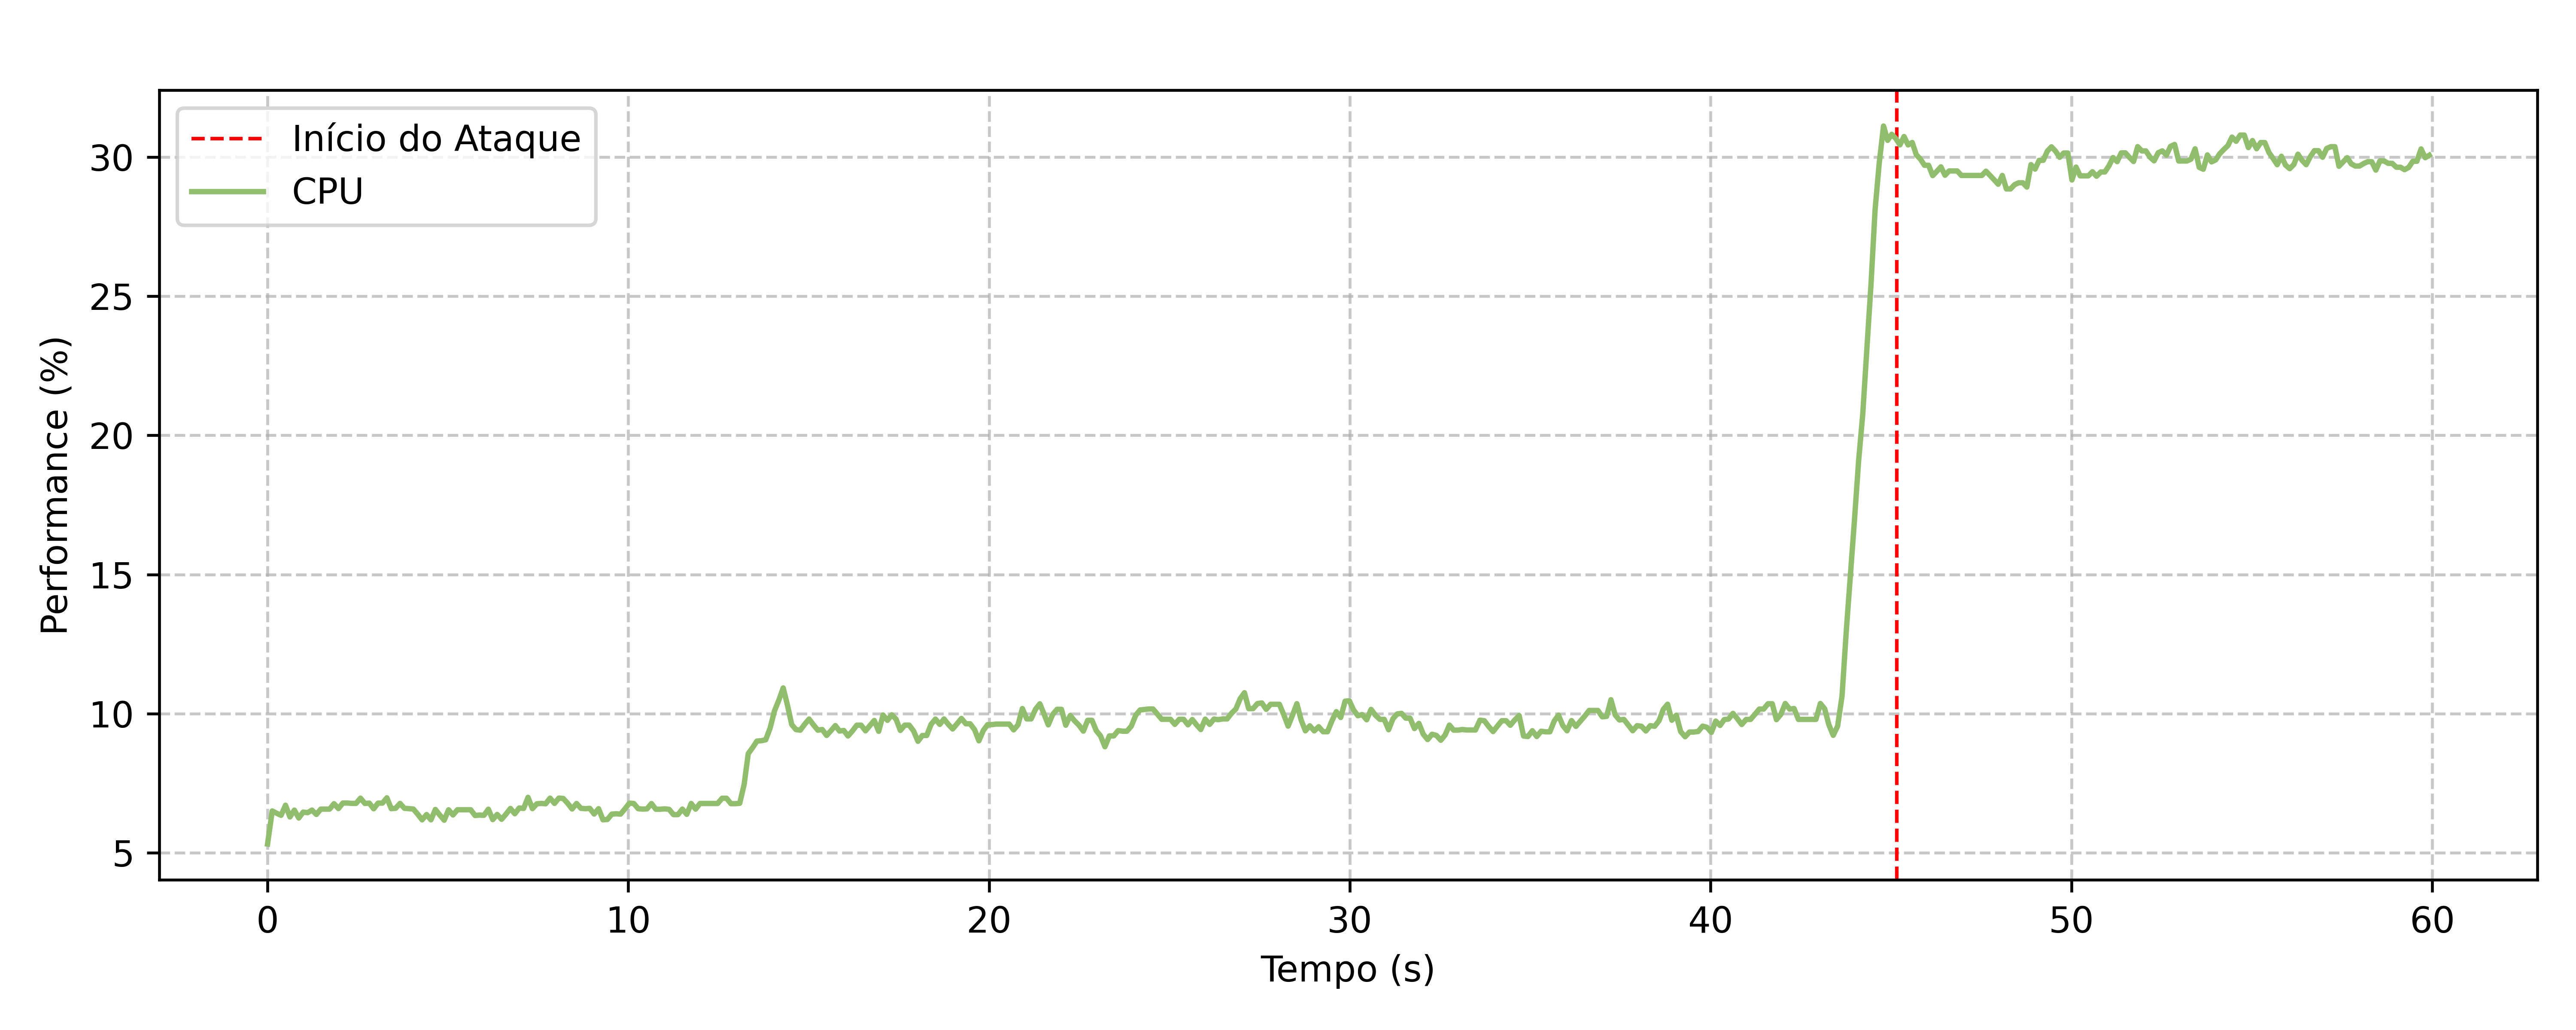
\includegraphics[width=1\textwidth]{USPSC-img/2-dos-hping-cpu.png}
                \end{subfigure}%
                \legend{Fonte: elaborada pelo autor.}
            \end{figure}

            Em média, o aumento de 275\% no uso do processamento no início do ataque, independentemente da configuração de segurança, evidencia a alta vulnerabilidade do servidor OPC UA a ataques de inundação TCP/IP. Esse comportamento foi observado em um ambiente controlado, no qual nenhuma outra tarefa estava sendo processada pelo controlador, permitindo isolar os efeitos do ataque. A elevada carga de tráfego gerada pode resultar na degradação do serviço, interrupção da comunicação e perda de dados críticos. Portanto, a implementação de medidas de segurança robustas é essencial para mitigar esse tipo de ameaça, assegurando a disponibilidade e a integridade dos sistemas industriais.

            No entanto, é importante destacar que esse ataque não foi direcionado especificamente ao protocolo OPC UA, mas sim à camada de transporte (quarta camada do modelo OSI). Embora a comunicação OPC UA não seja diretamente comprometida, a deterioração da infraestrutura de rede subjacente pode impactar significativamente sua funcionalidade, especialmente em ambientes industriais, onde a disponibilidade e a confiabilidade são requisitos fundamentais.

        \subsubsection*{\underline{Loop infinito na cadeia de certificados}}

            A tecnologia OPC UA demonstrou considerável resiliência ao ataque de negação de serviço baseado em loop infinito na cadeia de certificados. Essa análise pode ser realizada com base nos gráficos de RTT da comunicação. A Figura \ref{fig:0-dos-cert-rttp} apresenta a variação média do RTT normalizado por pacote durante a execução do ataque no cenário C3.

            \begin{figure}[htbp!]
                \caption{\label{fig:0-dos-cert-rttp}Tempo de ida e volta normalizado por pacote durante o ataque de loop infinito na cadeia de certificados - nível de segurança: `Sign \& Encrypt'}
                \begin{center}
                    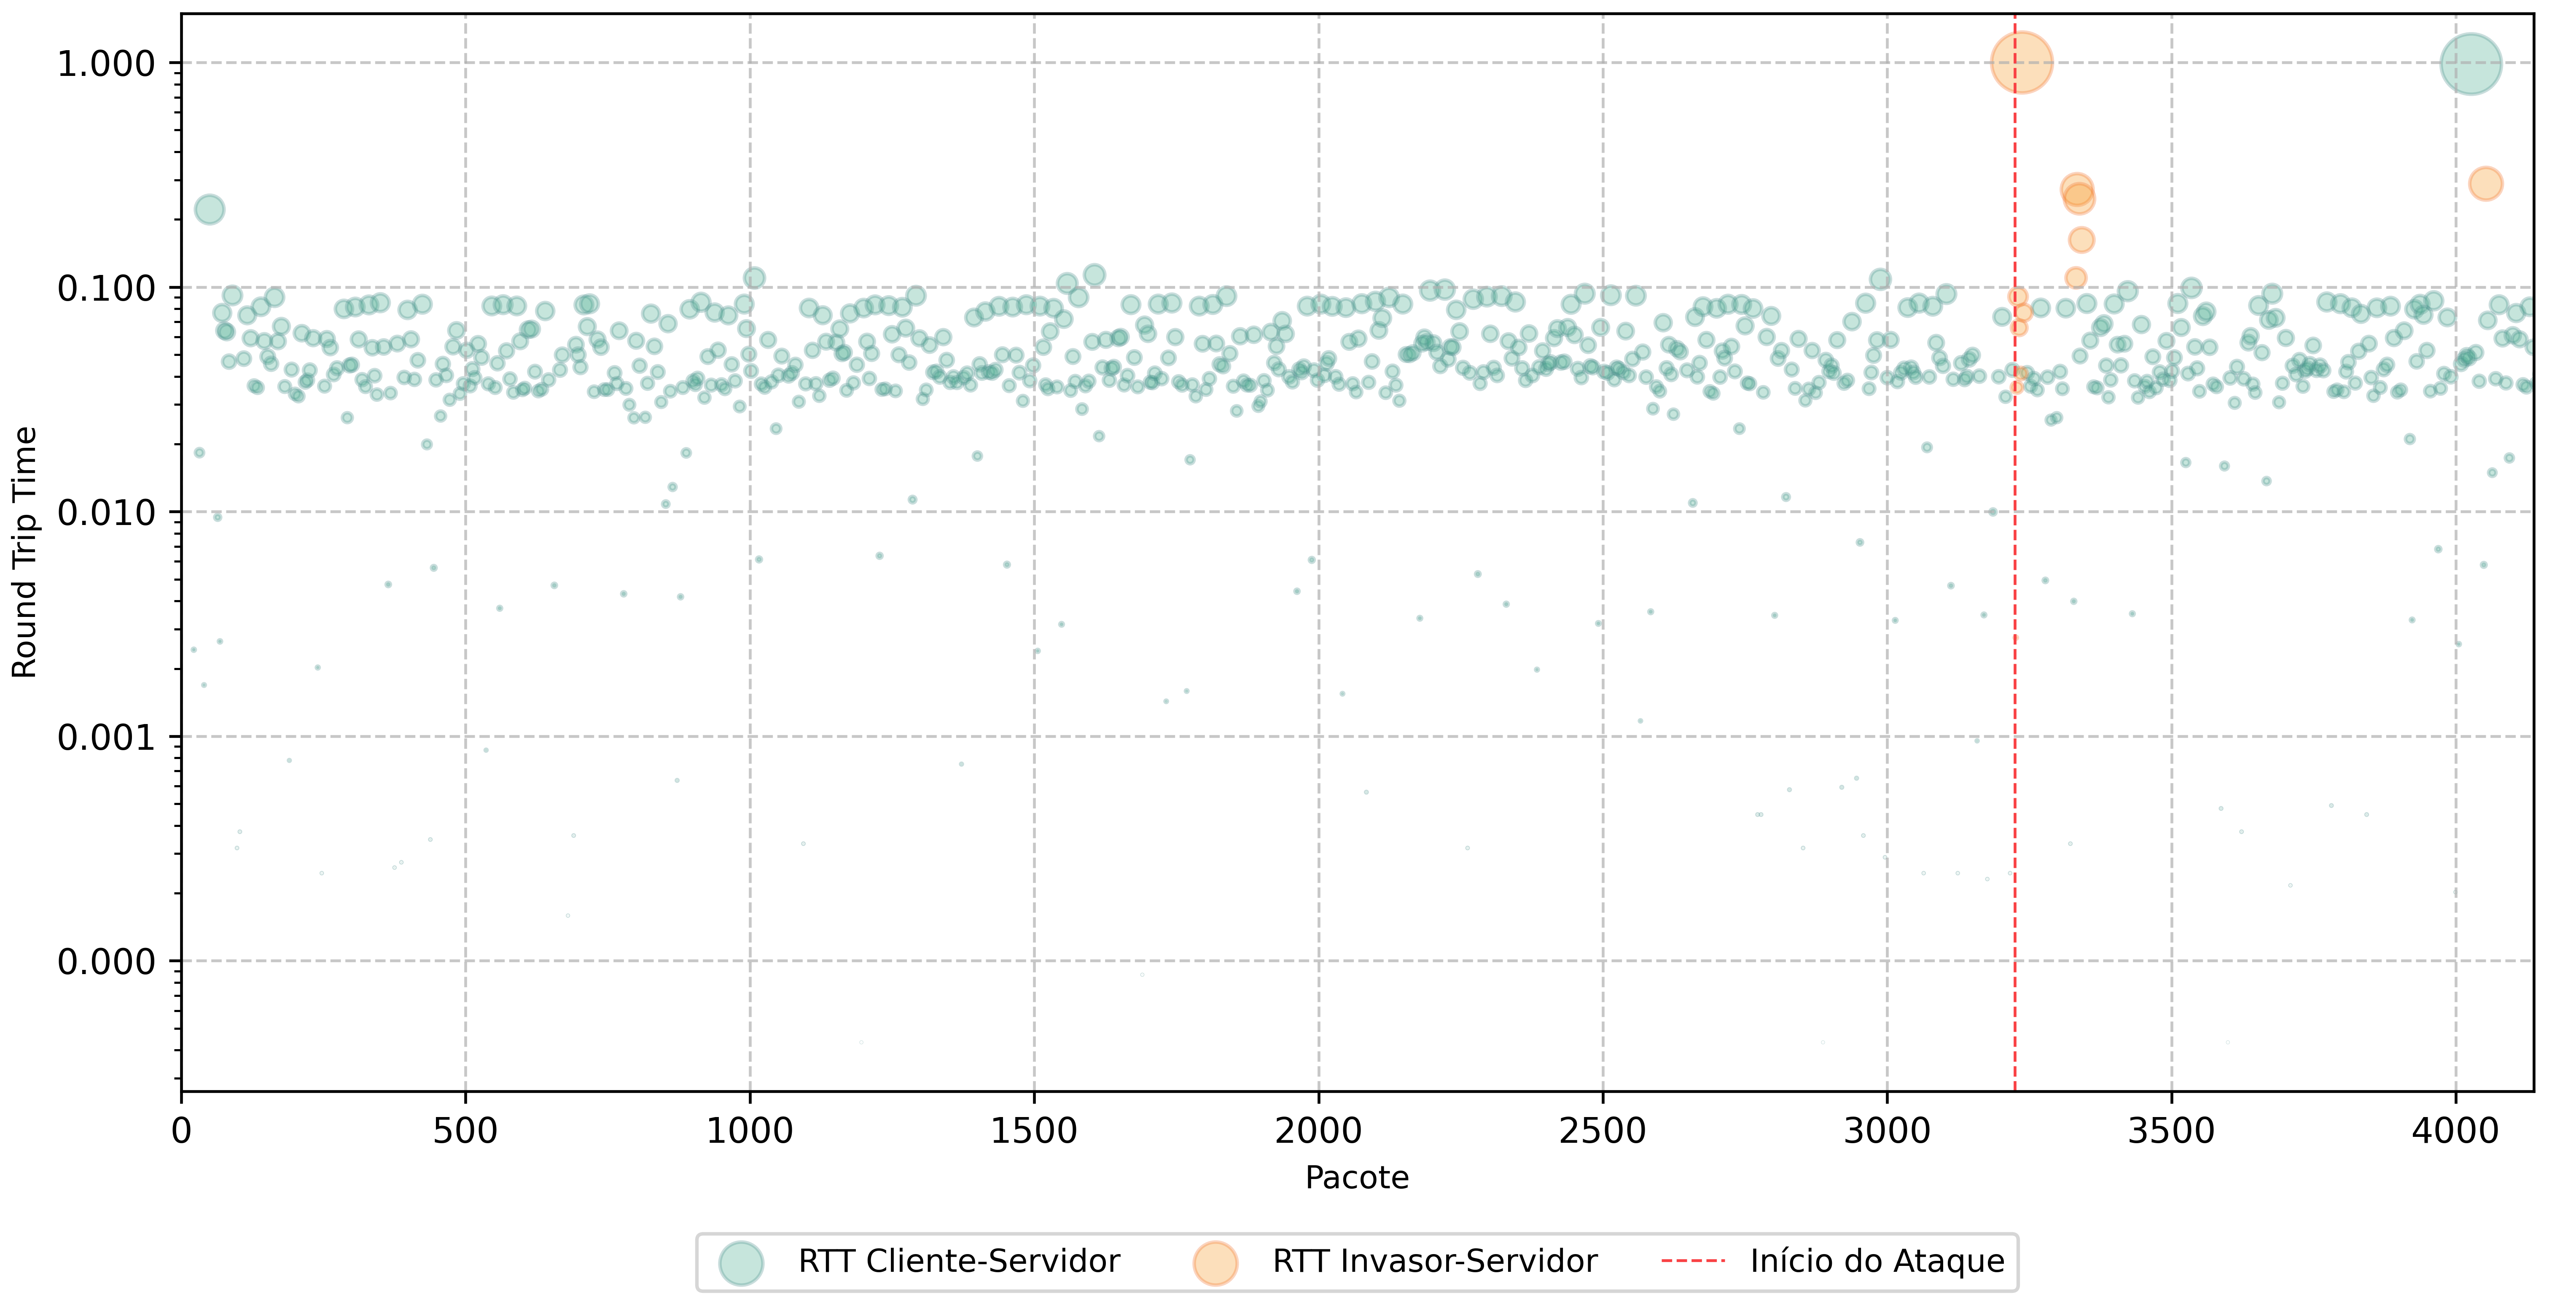
\includegraphics[width=0.972\textwidth]{USPSC-img/output/cropped/2-dos_certificate_inf_chain_loop-rttp.png}
                \end{center}
                \legend{Fonte: elaborada pelo autor.}
            \end{figure}

            A análise dos resultados revela que o invasor interage com o servidor OPC UA apenas no estágio inicial do ataque. A partir desse momento, a comunicação é interrompida para todos os modos de segurança, conforme indicado pela linha vermelha pontilhada que marca o início do ataque. Antes desse evento, o RTT Cliente-Servidor permanece constante e estável. No entanto, após o ataque, observa-se um aumento no RTT Invasor-Servidor, indicando que o servidor está sendo sobrecarregado com solicitações, resultando em um tempo de resposta mais elevado.

            O gráfico também evidencia uma dispersão significativa dos valores de RTT Invasor-Servidor após o início do ataque, sugerindo variações na capacidade do servidor de processar pacotes sob carga elevada. Entretanto, o RTT Cliente-Servidor apresenta pouca variação, demonstrando que o servidor consegue preservar a qualidade do serviço para comunicações legítimas, apesar da sobrecarga imposta pelo ataque.

            Essa análise reforça a robustez do protocolo OPC UA contra ataques de negação de serviço, especialmente em cenários onde são adotadas medidas de segurança avançadas, como criptografia e autenticação adequadas. Além disso, destaca a importância do monitoramento contínuo do desempenho do servidor e da implementação de mecanismos de mitigação para garantir a continuidade operacional e a integridade dos dados.

        \subsubsection*{\underline{Desreferenciação de ponteiro nulo}}

            O ataque de DoS por desreferenciação de ponteiro nulo revelou-se o único capaz de causar uma negação de serviço completa na rede OPC UA industrial em todos os cenários analisados (C4, C5 e C6). Esse ataque explora uma vulnerabilidade crítica no servidor, na qual uma chamada de função é executada sem a devida verificação da validade do ponteiro, resultando em uma falha que pode levar à interrupção total do serviço. A técnica baseia-se na tentativa de acessar ou modificar um ponteiro cujo valor é nulo, ou seja, não aponta para uma localização válida na memória. Como consequência, o programa tenta ler ou escrever em uma área de memória inválida, resultando em uma interrupção abrupta do funcionamento do sistema. A gravidade dessa falha reside no fato de que, além de comprometer a disponibilidade do serviço, ela pode ser explorada por atacantes para comprometer a segurança e a integridade do sistema. Dependendo do contexto, vulnerabilidades desse tipo podem permitir a execução de código malicioso ou causar a completa negação de serviço, como observado neste caso.

            A análise dos gráficos apresentados na \autoref{fig:2-dos_null_deref} permite uma compreensão detalhada do impacto desse ataque, considerando a rede configurada com o modo de segurança `Sign \& Encrypt'.

            \begin{figure}[htbp!]
                \centering
                \caption{\label{fig:2-dos_null_deref}Gráficos do ataque de DoS por desreferenciação de ponteiro nulo - nível de segurança: `Sign \& Encrypt'.}
                \begin{subfigure}[t]{0.5\textwidth}
                    \centering
                    \caption{\label{fig:2-dos_null_deref-tput}\textit{Throughput}}
                    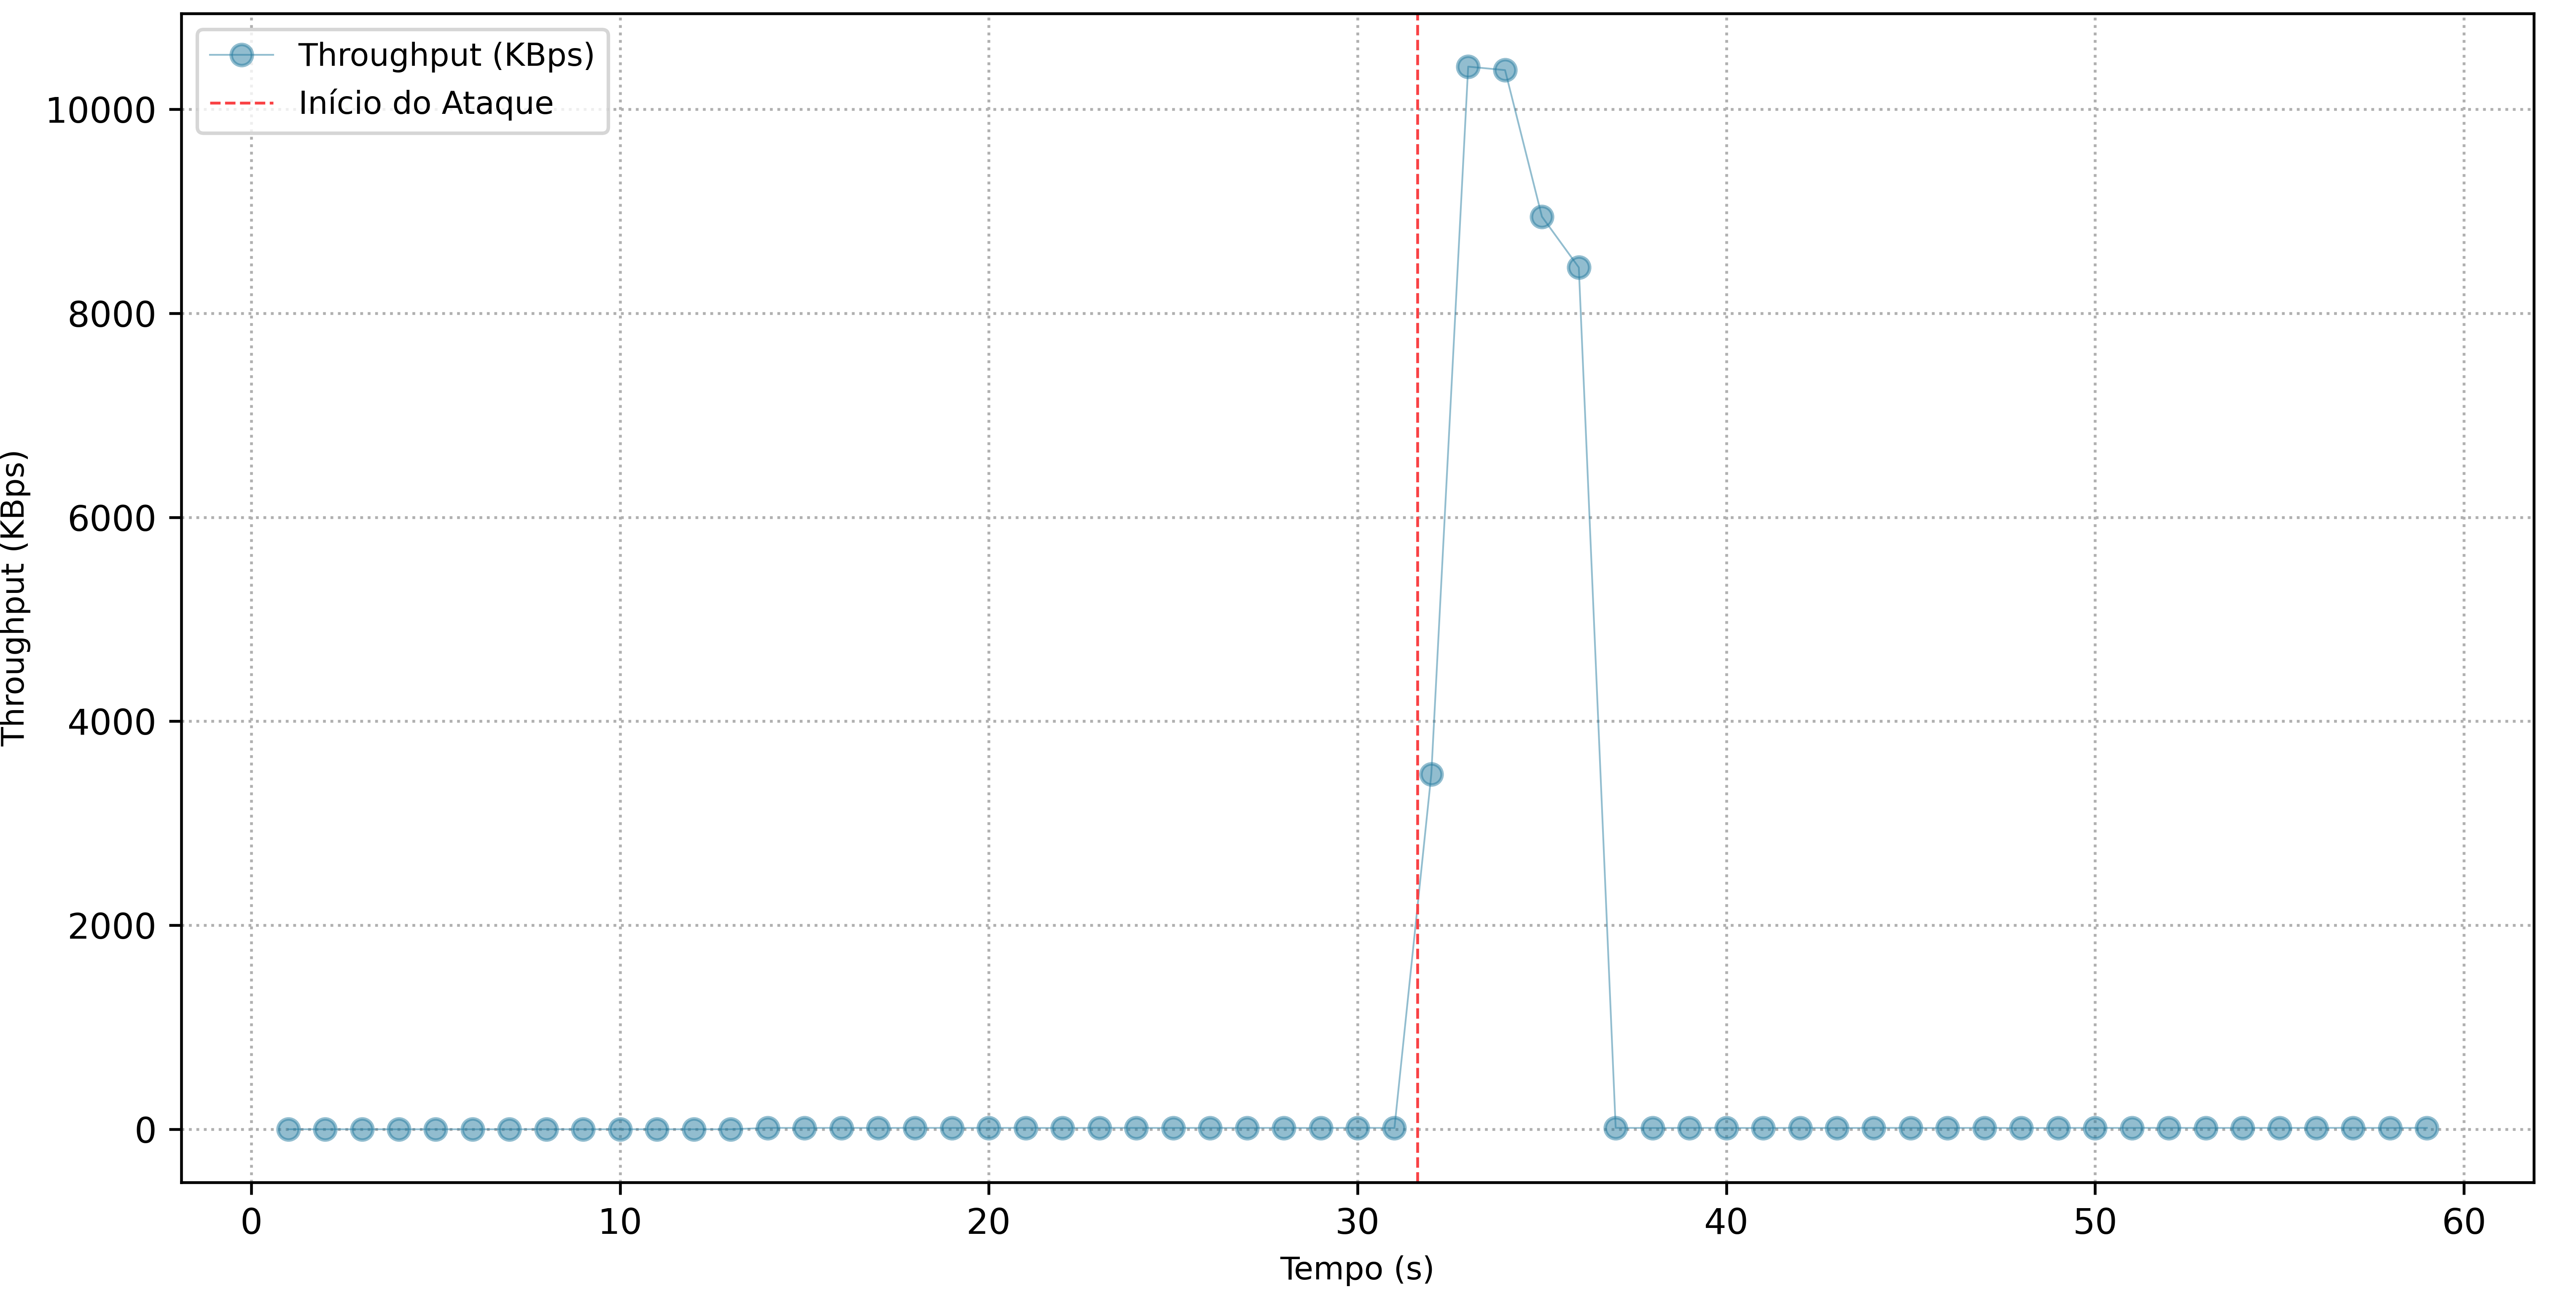
\includegraphics[width=1\textwidth, height=120pt]{USPSC-img/output/cropped/2-dos_function_call_null_deref-tput.png}
                \end{subfigure}%
                ~ 
                \begin{subfigure}[t]{0.5\textwidth}
                    \centering
                    \caption{\label{fig:2-dos_null_deref-perf}Desempenho}
                    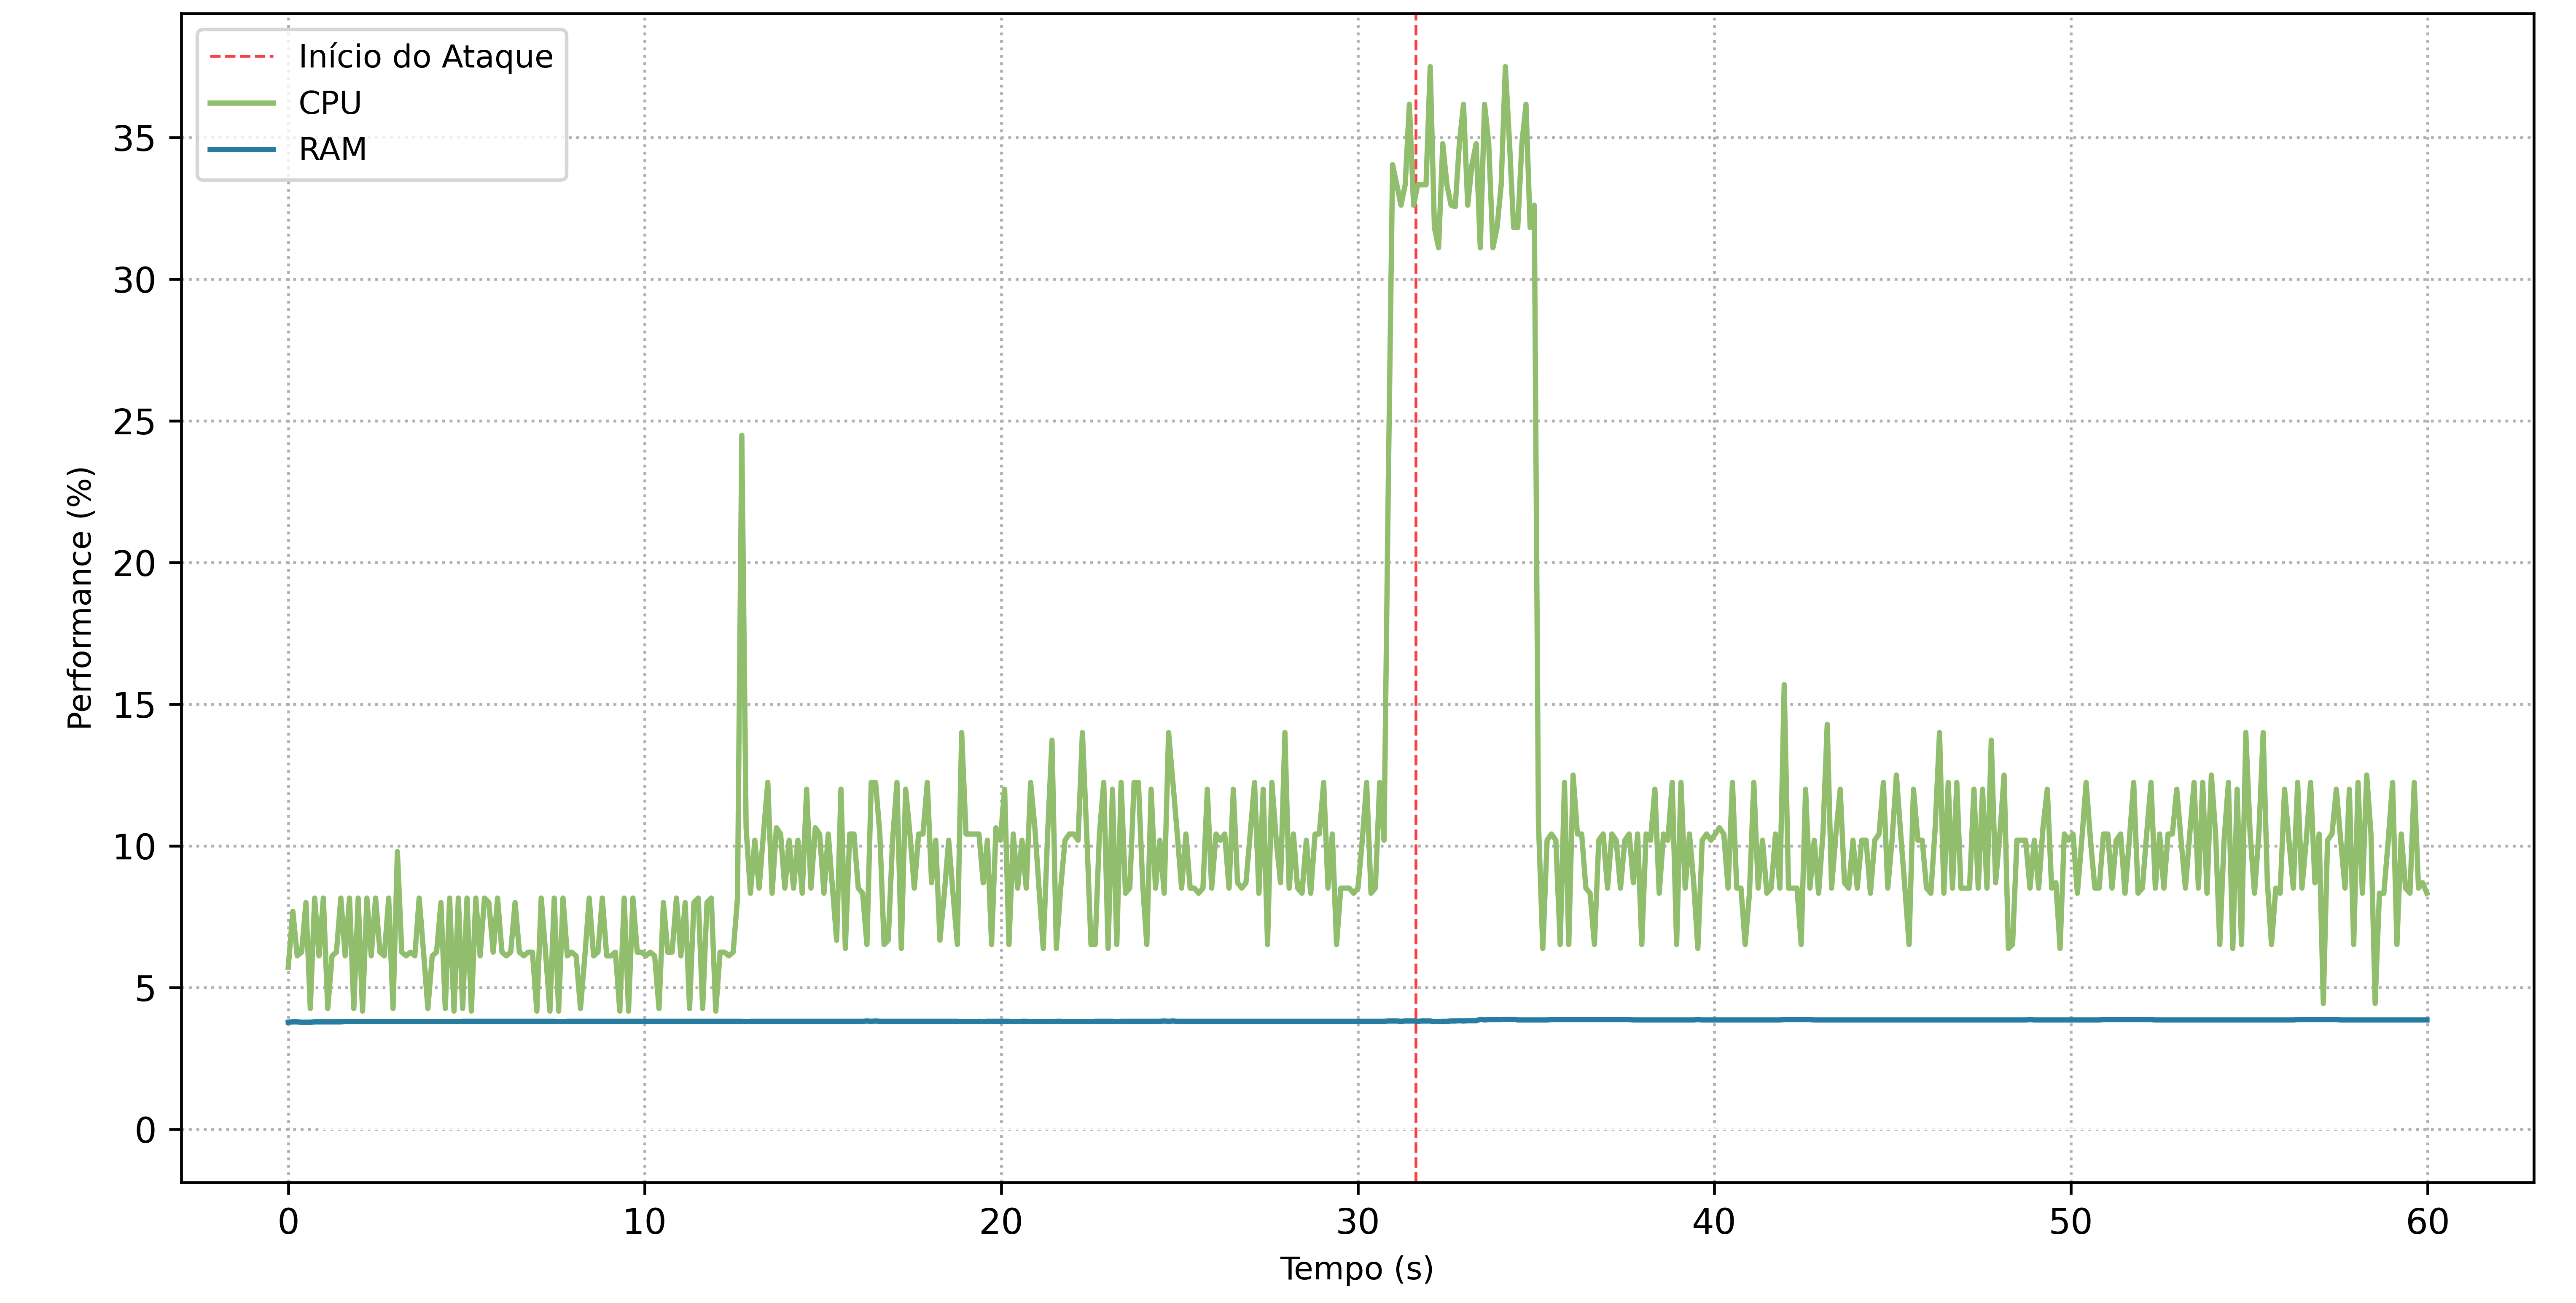
\includegraphics[width=1\textwidth, height=120pt]{USPSC-img/output/cropped/2-dos_function_call_null_deref-perf.png}
                \end{subfigure}%
                \\
                \begin{subfigure}[t]{0.5\textwidth}
                    \centering
                    \caption{\label{fig:2-dos_null_deref-pack}Pacotes OPC UA}
                    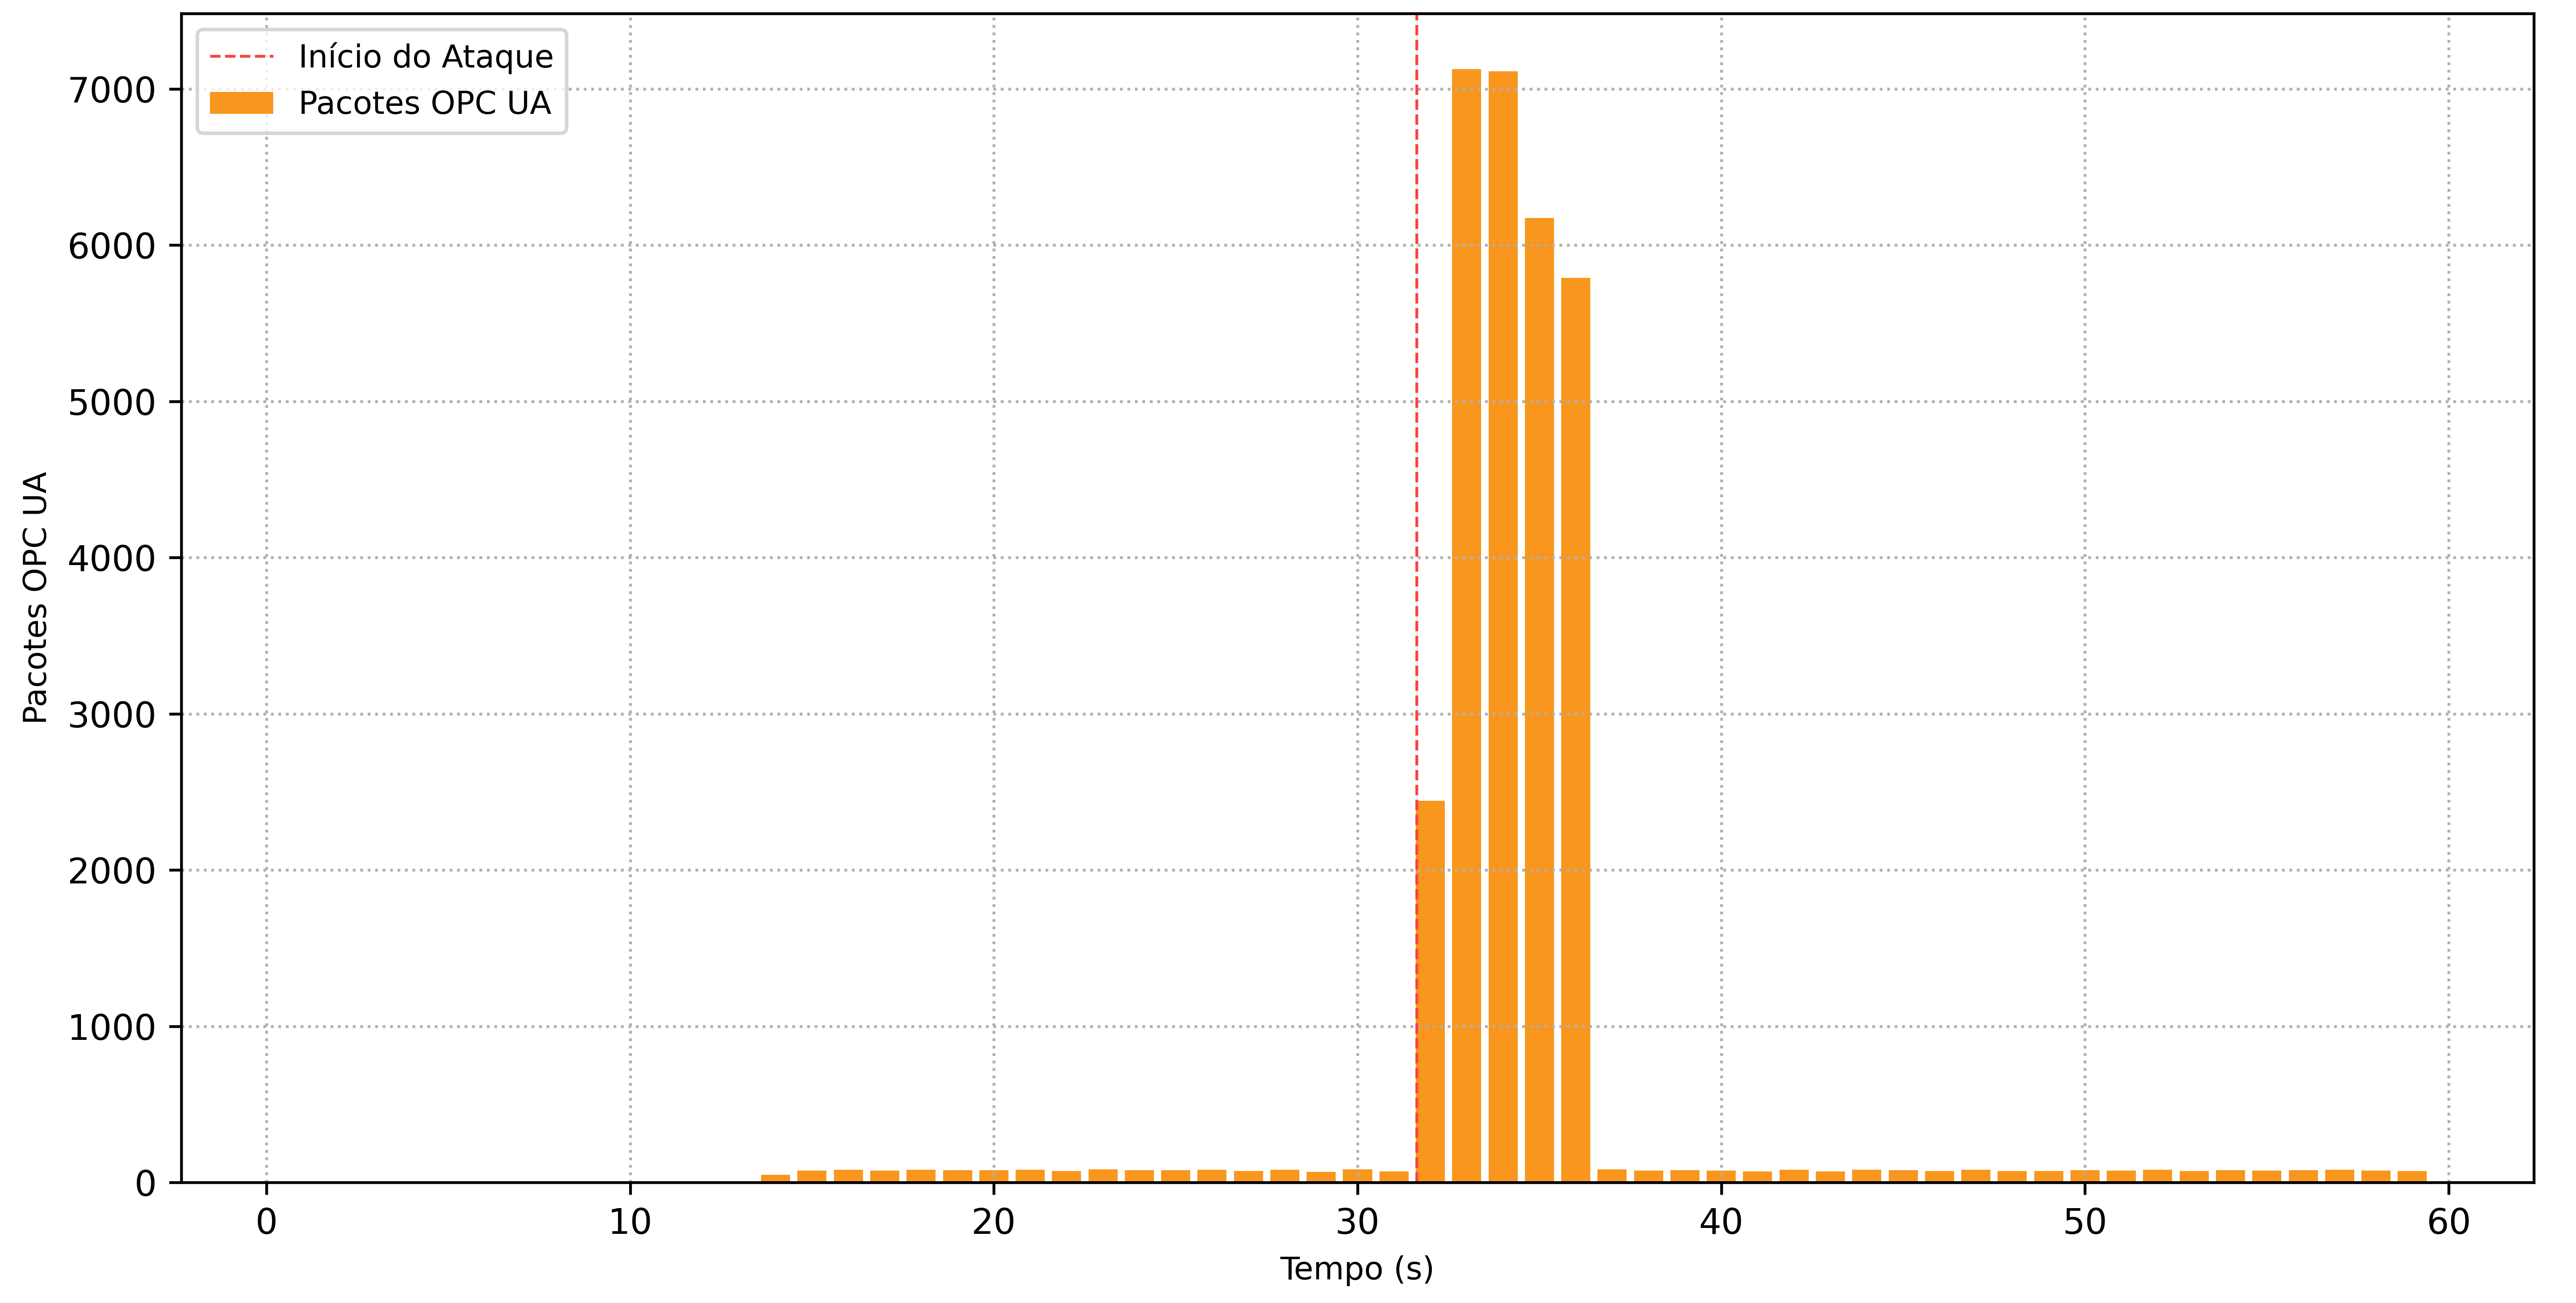
\includegraphics[width=1\textwidth, height=120pt]{USPSC-img/output/cropped/2-dos_function_call_null_deref-pack.png}
                \end{subfigure}%
                ~
                \begin{subfigure}[t]{0.5\textwidth}
                    \centering
                    \caption{\label{fig:2-dos_null_deref-rttp}RTT por pacote}
                    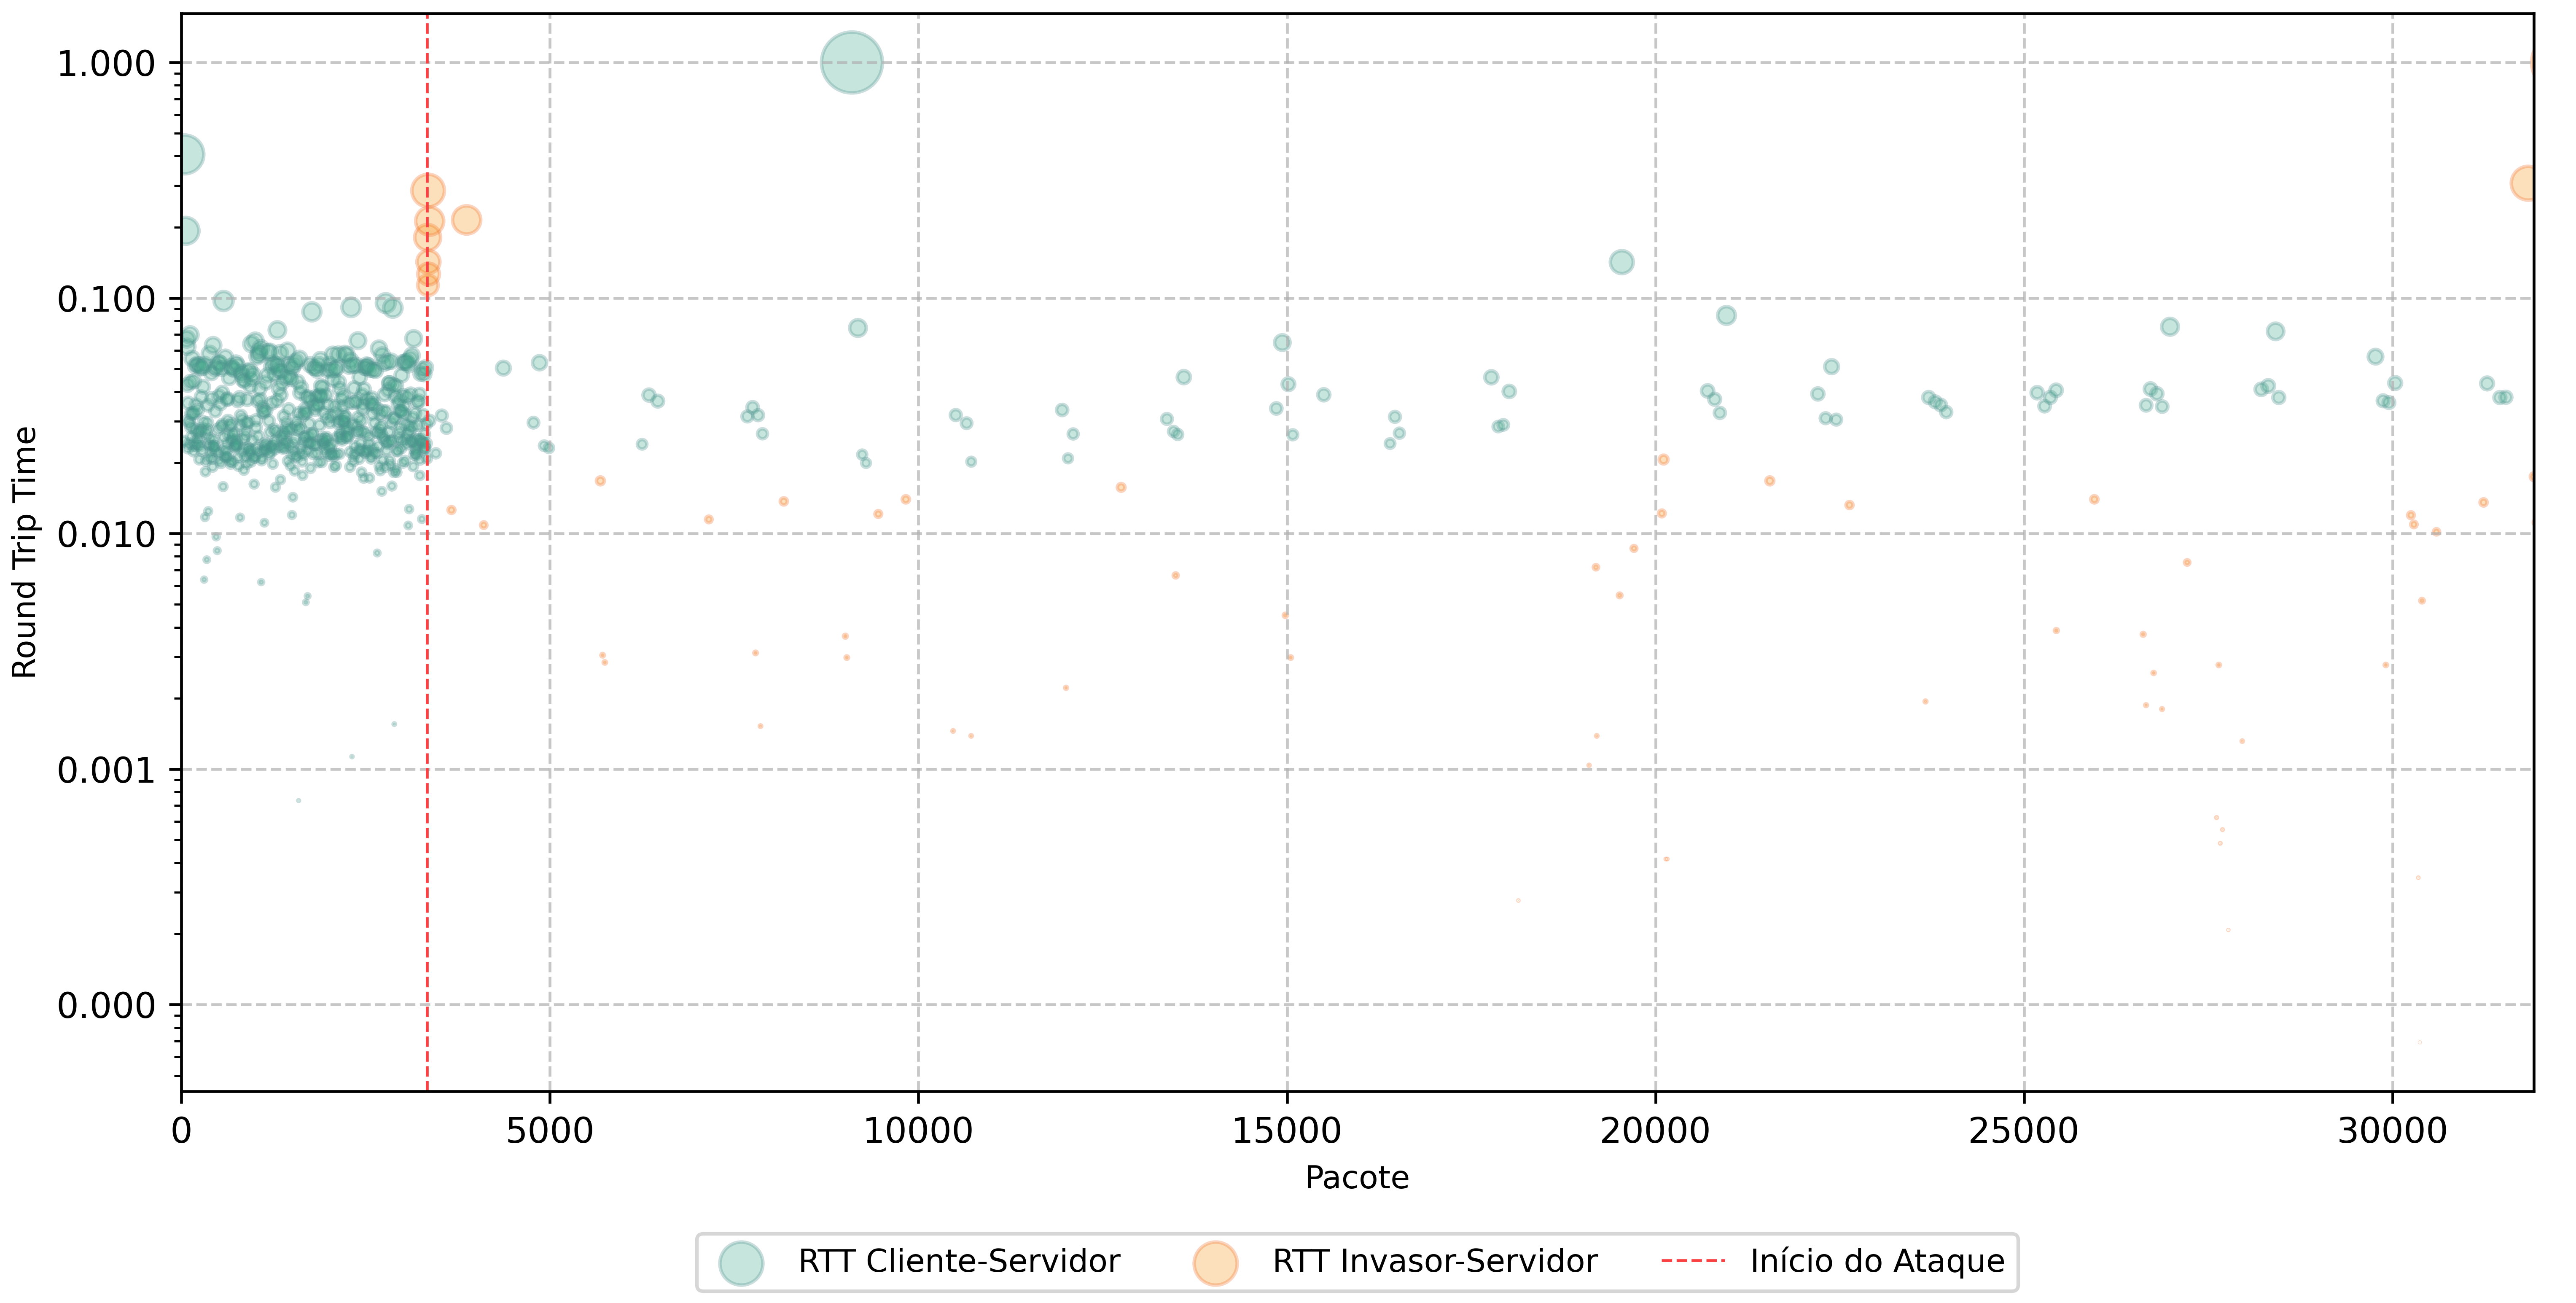
\includegraphics[width=1\textwidth, height=120pt]{USPSC-img/output/cropped/2-dos_function_call_null_deref-rttp.png}
                \end{subfigure}%
            \end{figure}

            O gráfico da taxa de transferência, representado na \autoref{fig:2-dos_null_deref-tput}, demonstra estabilidade em níveis baixos antes do ataque. Com o início do ataque, indicado pela linha vermelha, observa-se um aumento abrupto no \textit{throughput}, atingindo um pico significativo antes de cair drasticamente a zero. Esse comportamento indica que o servidor OPC UA foi sobrecarregado por solicitações inválidas, resultando em uma falha completa da comunicação, caracterizando a negação de serviço.

            A análise do gráfico do tempo de ida e volta por pacote, ilustrado na \autoref{fig:2-dos_null_deref-rttp}, reforça esses achados. Antes do ataque, o RTT entre cliente e servidor mantém-se relativamente constante, refletindo uma comunicação estável. No entanto, com o início do ataque, observa-se um aumento significativo no RTT, especialmente na comunicação entre o invasor e o servidor. Esse crescimento súbito sugere que o servidor está demorando mais para processar as solicitações devido à sobrecarga imposta pelo ataque, culminando no colapso da comunicação.

            O impacto do ataque no desempenho do servidor torna-se ainda mais evidente na \autoref{fig:2-dos_null_deref-perf}, que apresenta a utilização de CPU e memória RAM. Antes do ataque, o uso da CPU permanece em níveis baixos e constantes, indicando um funcionamento normal do servidor. No entanto, com o início do ataque, a utilização da CPU aumenta drasticamente, enquanto a ocupação da RAM se mantém estável. Esse crescimento abrupto no uso da CPU indica que o servidor está sobrecarregado ao tentar processar a grande quantidade de solicitações inválidas geradas pelo ataque, levando à degradação do desempenho e, eventualmente, à falha do sistema.

            Os resultados evidenciam que o ataque por desreferenciação de ponteiro nulo é altamente eficaz na exploração de vulnerabilidades específicas do servidor OPC UA, resultando em uma negação de serviço completa. A incapacidade do servidor de validar a integridade dos ponteiros antes da execução de funções críticas foi o principal fator que permitiu o sucesso do ataque. O rápido aumento na utilização da CPU e a subsequente falha na comunicação ressaltam a necessidade urgente de medidas de mitigação para proteger servidores OPC UA contra esse tipo de vulnerabilidade.


        \subsubsection*{\underline{Abertura de múltiplos canais seguros}}

            A análise dos ataques de DoS por meio de solicitações de abertura de múltiplos canais seguros na comunicação OPC UA evidencia uma vulnerabilidade crítica com potencial para comprometer redes industriais. Esse ataque explora a limitação do servidor OPC UA em gerenciar simultaneamente um grande número de requisições, resultando em sobrecarga e, eventualmente, na interrupção do serviço.

            Os resultados experimentais demonstram que a abertura simultânea de múltiplos canais seguros provoca um aumento significativo no \textit{throughput}, no tempo de resposta e na utilização da CPU. A \autoref{fig:0-dos-open-tput} ilustra que, logo após o início do ataque, o servidor tenta processar o volume excessivo de requisições; no entanto, sua capacidade de processamento se revela insuficiente para sustentar a eficiência operacional, levando a um estado de sobrecarga. Como consequência, observa-se um impacto adverso expressivo no RTT e no desempenho geral do host após o início do ataque.        

            \begin{figure}[htbp!]
                \caption{\label{fig:0-dos-open-tput}Taxa de transferência durante o ataque de abertura de múltiplos canais seguros - nível de segurança: `Sign'}
                \begin{center}
                    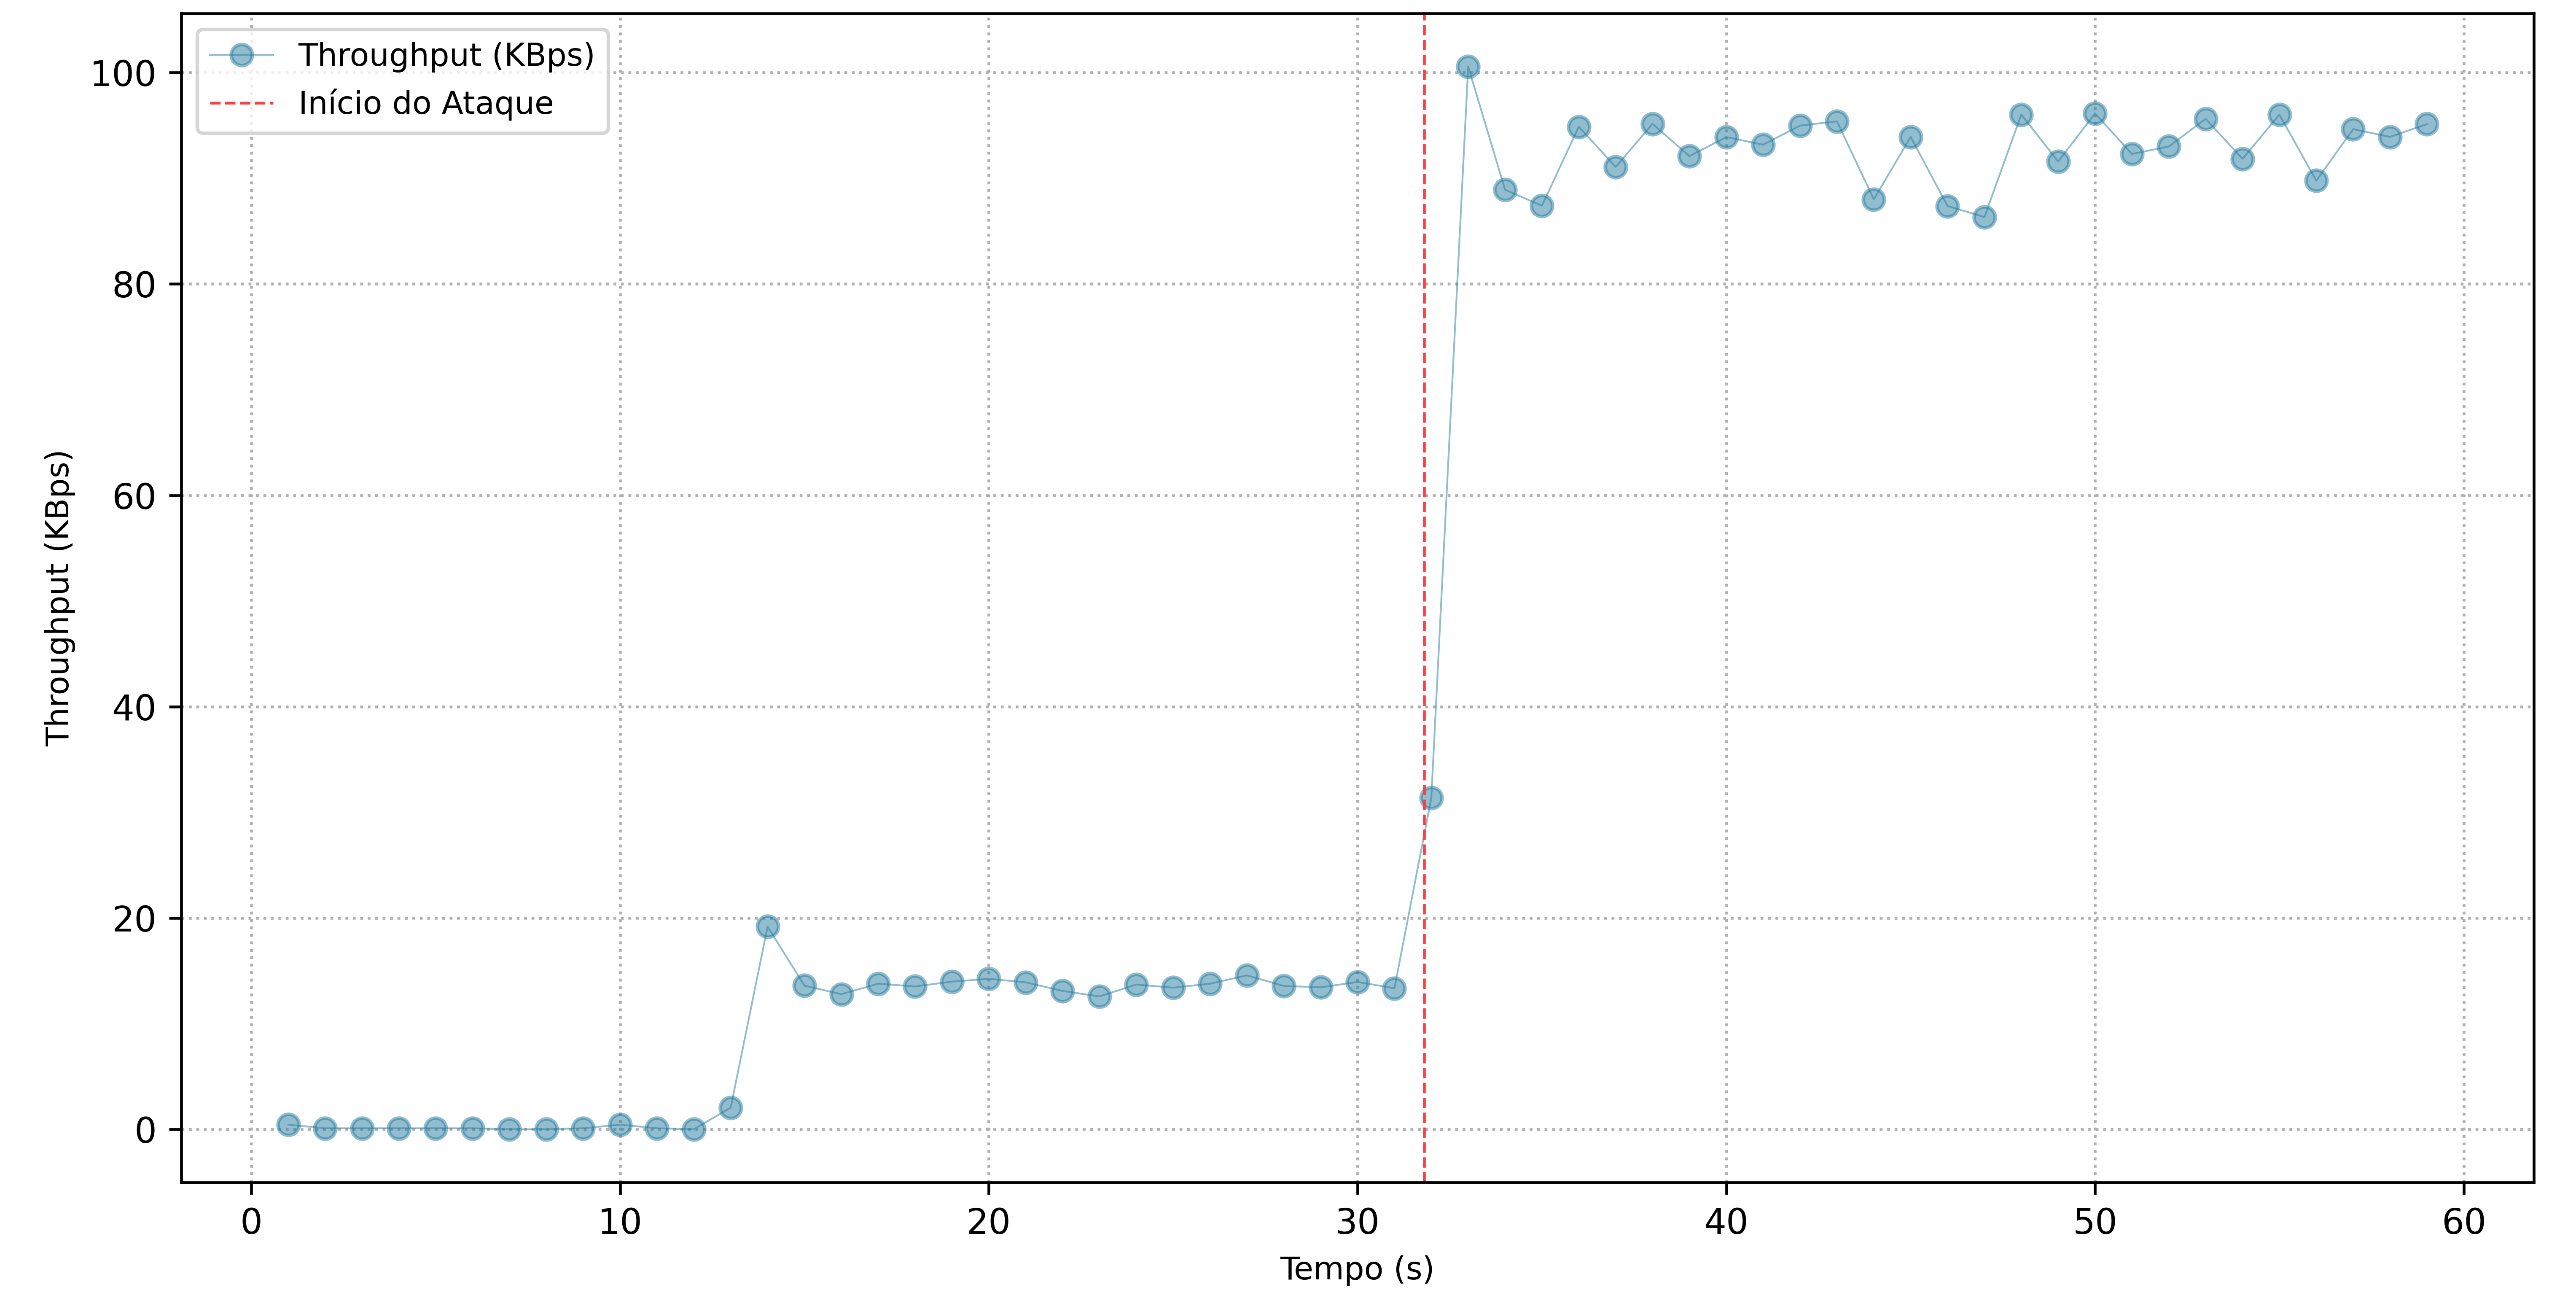
\includegraphics[width=0.972\textwidth]{USPSC-img/output/cropped/1-dos_open_multiple_secure_channels-tput.png}
                \end{center}
                \legend{Fonte: elaborada pelo autor.}
            \end{figure}

        \subsubsection*{\underline{Tradução do caminho de navegação}}

            Uma vulnerabilidade crítica que pode ser explorada para comprometer a estabilidade e a segurança da rede OPC UA é a exaustão da pilha da função responsável pelo processamento de requisições de tradução de caminhos de navegação para \texttt{NodeIds} (\texttt{TranslateBrowsePathsToNodeIds}). A função \texttt{TranslateBrowsePath} executa a conversão de caminhos de navegação (do inglês, \textit{browse paths}) em \texttt{NodeIds}. Durante esse processo, a função é chamada recursivamente para cada elemento no caminho relativo (\texttt{RelativePath}), sem a imposição de um limite adequado para a profundidade da recursão. Como consequência, a tradução de um caminho de navegação excessivamente longo pode resultar em uma exceção de estouro de pilha (\texttt{StackOverflowException}).

            Entretanto, a análise dos resultados obtidos nos cenários C13, C14 e C15 indica que a rede OPC UA possui uma proteção parcial contra ataques de negação de serviço por exaustão da pilha. A avaliação dos gráficos de tráfego da rede, especialmente a análise do tempo de resposta do servidor, revela uma degradação progressiva no desempenho do sistema, evidenciada pelo aumento expressivo desse tempo à medida que o número de requisições maliciosas foi incrementado.        

\section{Propostas de Melhorias e Mitigações} \label{sec:melhorias-mitigacoes}

    A melhoria da resiliência cibernética de um IACS deve ser um dos principais benefícios da implementação de um programa de segurança industrial. Essa resiliência é alcançada por meio da seleção criteriosa de controles de segurança, os quais devem abranger um processo contínuo de abordagem à cibersegurança. Esse processo não se limita à dissuasão e prevenção de ameaças, mas também deve equilibrar de forma adequada a detecção e a correção de incidentes. Essa estratégia gerencial é essencial para identificar eventos cibernéticos de maneira oportuna e responder adequadamente, minimizando as consequências e restaurando a operação normal da instalação de manufatura.

    As organizações frequentemente alocam grande parte de seu orçamento de segurança em mecanismos de prevenção de ataques. No entanto, muitas vezes são alertadas por partes externas sobre a falta de investimentos equilibrados em controles de detecção de incidentes, o que pode ocorrer muito tempo após a materialização de um ataque. A segurança deve ser tratada como um investimento estratégico de longo prazo, em vez de uma despesa tática e pontual. Investidores e gestores de instalações industriais compreendem o ciclo de vida prolongado dos investimentos de capital, tornando coerente que a segurança industrial destinada à proteção dessas instalações receba atenção contínua e um orçamento compatível, assim como outras despesas operacionais, incluindo manutenção, aprimoramentos e treinamento.

    Nesta seção, apresentam-se as propostas de melhorias e mitigações identificadas, organizadas em duas categorias principais: recomendações para comunicações seguras com o protocolo OPC UA e aprimoramentos na infraestrutura e gestão de redes. Adicionalmente, na última subseção, são descritas as normas e regulamentações que podem ser empregadas para garantir a conformidade com os requisitos de segurança industrial. A implementação dessas recomendações visa não apenas aumentar a robustez das comunicações, mas também assegurar a continuidade das operações industriais de forma segura e eficiente.

    \subsection{Recomendações para Comunicações Seguras com o Protocolo OPC UA}

        Especialmente no contexto do protocolo OPC UA, uma série de testes conduzidos em conformidade com os padrões de segurança identificou diversas recomendações para mitigar vulnerabilidades e fortalecer a integridade, a disponibilidade e a confidencialidade dos dados.

        Em primeiro lugar, assim como em qualquer outro software ou protocolo, a atualização regular é fundamental para garantir a segurança do OPC UA. De modo geral, atualizações incluem correções de \textit{bugs} e \textit{patches} de segurança projetados para mitigar vulnerabilidades conhecidas. Portanto, recomenda-se que todo o IACS seja mantido atualizado, abrangendo sistemas operacionais, aplicativos, bibliotecas e protocolos, incluindo o OPC UA.

        Além disso, a seleção de um modo de segurança adequado deve considerar os requisitos específicos do sistema e a sensibilidade dos dados transmitidos. O modo de assinatura e criptografia (`Sign \& Encrypt) não apenas assegura a integridade dos dados, mas também garante sua confidencialidade, prevenindo a interceptação e a modificação não autorizada das informações. A escolha dos algoritmos criptográficos dentro dessa configuração desempenha um papel central na segurança das comunicações OPC UA. Como o protocolo suporta diferentes políticas de segurança, as organizações devem priorizar aquelas que oferecem proteção robusta e estejam alinhadas com seus requisitos de segurança e padrões de conformidade.

        No que se refere à autenticação de usuários, é essencial evitar o uso de credenciais anônimas para acessar recursos críticos. O uso de um ID anônimo inviabiliza o rastreamento de alterações em dados ou configurações, criando brechas para atividades não autorizadas. Dessa forma, devem ser aplicadas restrições rigorosas ao uso de identificadores anônimos, limitando sua utilização exclusivamente a operações não críticas. Além disso, o compartilhamento de credenciais entre usuários ou sistemas aumenta o risco de comprometimento de dados e roubo de identidade. A adoção da autenticação multifator, combinada com políticas de senhas robustas, fortalece ainda mais a segurança ao adicionar camadas adicionais de verificação.

        A proteção das chaves privadas e dos certificados é outro aspecto crítico. Esses elementos não devem ser armazenados em sistemas de arquivos não criptografados, dada sua alta sensibilidade. Uma alternativa recomendada é delegar a gestão de chaves a um serviço especializado (KMS, do inglês \textit{Key Management Service}) ou utilizar sistemas operacionais que permitam a definição de direitos de acesso apropriados. Adicionalmente, o uso de TPMs (\textit{Trusted Platform Modules}) ou de dispositivos de \textit{hardware} seguro, como tokens de autenticação USB, é altamente recomendado para o armazenamento seguro de certificados e chaves privadas, reduzindo significativamente o risco de comprometimento desses ativos. Conexões que utilizem certificados não confiáveis devem ser bloqueadas, uma vez que certificados autoassinados, embora compatíveis com a comunicação OPC UA, exigem verificações adicionais. O ideal é estabelecer uma autoridade certificadora (CA, do inglês \textit{Certificate Authority}), garantindo que seus certificados sejam assinados por uma entidade independente ou por outra CA em um modelo de confiança multinível, reforçando a autenticidade das comunicações.

        Além das medidas mencionadas, é fundamental habilitar a auditoria e o registro de eventos em todos os sistemas OPC UA. Esse mecanismo permite o rastreamento detalhado e o monitoramento contínuo de acessos e atividades no servidor, possibilitando a rápida identificação de incidentes de segurança e a detecção de anomalias no comportamento do sistema. Além de fortalecer a postura de segurança da organização, a auditoria contribui para o cumprimento de requisitos regulatórios relacionados à proteção de dados e ao controle de acesso. A existência de registros detalhados e auditáveis é essencial para a responsabilização das ações realizadas dentro do sistema, viabilizando respostas eficazes a potenciais incidentes de segurança.

        Por fim, a implementação de controles de acesso baseados em funções deve ser priorizada na gestão de usuários do OPC UA. O RBAC (\textit{Role-Based Access Control}) permite um controle rigoroso dos recursos do sistema com base nas funções e permissões atribuídas a cada usuário, aplicando o princípio do menor privilégio. Essa abordagem reduz significativamente o risco de acessos não autorizados e do uso indevido de privilégios, garantindo que os usuários disponham apenas das permissões estritamente necessárias para a execução de suas tarefas. A definição precisa de funções e permissões, alinhada aos requisitos de segurança e às necessidades operacionais da organização, é essencial para assegurar a integridade e a proteção do ambiente industrial.

    \subsection{Melhorias na Infraestrutura e Gestão de Redes}

        Para garantir a segurança e a resiliência das redes industriais OPC UA, torna-se essencial adotar estratégias de mitigação focadas na infraestrutura e na gestão da rede. A complexidade e a criticidade dos sistemas de automação e controle industrial demandam uma abordagem robusta e abrangente para a proteção contra ataques cibernéticos, como os discutidos neste trabalho. Dessa forma, apresentam-se algumas práticas e tecnologias que podem ser empregadas para fortalecer a infraestrutura de rede, prevenindo a interceptação e manipulação do tráfego, além da implementação de mecanismos de monitoramento eficazes para detectar e responder rapidamente a atividades suspeitas.

        Os ataques MITM, incluindo roubo de portas e falsificação da tabela ARP, podem ser mitigados por meio de diversas abordagens e melhorias na infraestrutura do IACS. A segurança de porta nos \textit{switches} é uma medida essencial para impedir que dispositivos não autorizados interceptem o tráfego de rede, limitando o número de endereços MAC que podem ser aprendidos em cada porta e desativando automaticamente aquelas que apresentem violações, aumentando, assim, a segurança da rede. Além disso, a utilização de entradas estáticas na tabela ARP impede que equipamentos maliciosos modifiquem esses dados para redirecionar o tráfego, sendo uma abordagem eficaz em redes onde a topologia e os endereços IP são conhecidos e estáveis.
        
        Adicionalmente, a implementação de monitoramento ativo e passivo é fundamental para detectar e responder a atividades suspeitas na rede. Ferramentas como \texttt{arpwatch} e \texttt{ettercap} permitem a identificação de alterações na tabela ARP e a interceptação de tráfego malicioso em tempo real. O monitoramento ativo, em particular, é crucial para identificar e mitigar ataques MITM em andamento, protegendo a integridade e a confidencialidade dos dados. A combinação dessas técnicas de monitoramento com a implementação de sistemas de detecção de intrusão fortalece a postura de segurança da rede, permitindo a identificação precoce de ameaças e a resposta rápida a incidentes.
        
        A criptografia de dados em trânsito, por meio de protocolos seguros como TLS/SSL, é essencial para proteger informações sensíveis contra acessos não autorizados. Mesmo que um invasor consiga capturar o tráfego por meio de técnicas de \textit{sniffing}, a criptografia garante que os dados capturados permaneçam ilegíveis e inoperantes sem a chave de decriptação correspondente.
        
        A segmentação de rede, implementada por meio de VLANs (do inglês \textit{Virtual Local Area Network}), é uma estratégia eficaz para limitar a exposição dos dados e controlar o tráfego da rede. Ao segmentar a rede em diferentes zonas, a comunicação entre dispositivos fica restrita apenas aos segmentos necessários, reduzindo significativamente o risco de acessos não autorizados. Essa abordagem dificulta a propagação de ameaças cibernéticas, como ataques laterais, e minimiza o impacto de eventuais incidentes de segurança.
        
        De acordo com \citeonline{knapp2024}, estabelecer a segurança de rede para proteger o acesso a uma zona definida requer a implementação de um rigoroso código de conduta. As regras de segurança devem estar em conformidade com os canais de comunicação contidos nesses condutos. Os controles de segurança de rede são projetados tanto para impedir acessos não autorizados aos sistemas internos quanto para evitar que esses sistemas se conectem a redes externas de maneira descontrolada. Para garantir a proteção efetiva do tráfego de entrada e saída, recomenda-se a adoção das seguintes medidas:
        
        \begin{enumerate}
            \item Todo o tráfego de entrada e saída deve ser canalizado por meio de uma ou mais conexões de rede confiáveis, que sejam continuamente monitoradas e controladas.
            \item Dispositivos de segurança devem ser instalados em linha em cada uma dessas conexões, podendo incluir funcionalidades de segurança incorporadas em \textit{switches} e roteadores da rede.
            \item Para cada zona, é crucial selecionar e implementar os dispositivos de segurança adequados, seguindo recomendações específicas para o contexto.
        \end{enumerate}    

        Dessa forma, a seleção dos dispositivos de segurança de rede é um aspecto fundamental na proteção das zonas definidas dentro de uma infraestrutura de controle industrial. Para assegurar a segurança, a implementação de firewalls é frequentemente considerada um requisito mínimo, sendo complementada, conforme a criticidade da zona, por IDS e dispositivos de prevenção de intrusão (IPS, do inglês \textit{Intrusion Prevention Systems}). A combinação de firewalls e IPS revela-se particularmente eficaz, pois enquanto os firewalls controlam o tráfego permitido, o IPS realiza uma análise aprofundada desse tráfego para identificar ameaças ocultas. Essa abordagem adiciona uma camada extra de proteção e reduz significativamente o risco de ataques DoS e DDoS.

        A microsegmentação é outra estratégia recomendada, pois possibilita um controle mais granular sobre a comunicação entre dispositivos, aplicações e usuários, facilitando a aplicação de políticas de segurança específicas para cada segmento da rede. Ademais, a diferenciação entre detecção e prevenção é essencial, sobretudo em redes industriais, onde a disponibilidade e o desempenho são prioritários. Nessas redes, o IDS é preferencialmente adotado dentro das zonas industriais, evitando a perda de pacotes devido a falsos positivos, enquanto o IPS é mais apropriado para os limites entre zonas industriais e empresariais, onde o impacto de eventuais interrupções pode ser melhor gerenciado.

        Além disso, a segurança dos dispositivos dentro dessas zonas é igualmente crítica, independentemente de estarem conectados à rede. Equipamentos que não podem ser protegidos por métodos tradicionais devem ser isolados em subzonas de segurança específicas, com condutos rigorosamente controlados. Mesmo dispositivos embarcados, que frequentemente apresentam vulnerabilidades, devem ser protegidos sempre que possível. Isso pode incluir a adoção de controles de segurança compensatórios nos condutos que interligam esses dispositivos às zonas mais amplas, garantindo a manutenção da segurança em todos os níveis da infraestrutura.

        Por fim, a proteção de dispositivos e aplicações dentro das zonas requer não apenas controle de acesso rigoroso, mas também um monitoramento contínuo das comunicações. Os dispositivos presentes nessas zonas, especialmente aqueles com interfaces de rede, devem ser protegidos por mecanismos robustos de autenticação, controle de acesso e manutenção adequada. O monitoramento das atividades dos dispositivos desempenha um papel crucial na detecção de possíveis ameaças e na garantia da eficácia das políticas de segurança. A implementação de SIEM é uma prática recomendada, pois permite a consolidação e análise centralizada de logs de segurança, viabilizando a identificação de padrões de tráfego suspeitos e a resposta rápida a incidentes de segurança.


    \subsection{Normas e Regulamentos}

        No contexto da segurança cibernética, diversos padrões, diretrizes e regulamentos são estabelecidos por governos e indústrias, variando desde as ``melhores práticas'' até requisitos rigorosos, cuja não conformidade pode resultar em penalidades e multas. Muitos desses documentos normativos abrangem a segurança da informação de forma geral; entretanto, a quantidade de publicações específicas para sistemas de automação e controle industrial tem aumentado significativamente. Segundo \citeonline{knapp2024}:

        \begin{citacao}
            Nos Estados Unidos, alguns padrões comuns abarcam os Padrões de Confiabilidade de Proteção de Infraestruturas Críticas (CIP) da North American Electric Reliability Corporation (NERC), os Padrões de Antiterrorismo para Instalações Químicas (CFATS) do Departamento de Segurança Interna dos EUA (DHS), a Regulamentação de Segurança de Instalações Nucleares pela Comissão Reguladora Nuclear dos EUA (NRC), além das recomendações gerais de segurança para IACS publicadas pelo Instituto Nacional de Padrões e Tecnologia (NIST) na Publicação Especial 800-82. Na Europa, normas e diretrizes incluem o EU M/490 e o SGCG, que fornecem orientações para sistemas de energia modernos, e diversas publicações da Agência Europeia para a Segurança das Redes e da Informação (ENISA). Padrões globais incluem a série de normas ISO/IEC 27000 da Organização Internacional de Normalização (ISO), das quais a ISO-27002:2013, ``Código de prática para controles de segurança da informação'', é amplamente adotada.
        \end{citacao}
        
        Entre os padrões mais relevantes para a segurança industrial, destaca-se a norma ISA/IEC 62443 (anteriormente denominada ISA 99), desenvolvida pela Sociedade Internacional de Automação (ISA, do inglês \textit{International Society of Automation}) em parceria com a Comissão Eletrotécnica Internacional (IEC, do inglês \textit{International Electrotechnical Commission}). Esse padrão foca na segurança de sistemas de automação e controle industrial e pode ser aplicado a qualquer organização ou setor que utilize tais sistemas. Os níveis de segurança definidos na norma visam proteger a confidencialidade das informações, organizando-os conforme a capacidade e os recursos de possíveis atacantes.

        A adoção de uma abordagem holística para a segurança é um dos princípios centrais da ISA/IEC 62443, enfatizando a necessidade de incorporar medidas de proteção desde a fase de concepção dos sistemas até sua implementação e manutenção. Esse conceito, conhecido como ``segurança desde o design'' (do inglês \textit{Secure by Design}), assegura que a proteção dos IACS não seja tratada como um complemento, mas como parte integrante do processo de desenvolvimento. Esse princípio pode ser efetivado por meio da defesa em profundidade, técnica baseada na implementação de múltiplas camadas de controles de segurança que combinam medidas físicas, técnicas e procedimentais para mitigar tanto ameaças externas quanto internas. Além disso, a norma destaca a necessidade de avaliações contínuas de risco para identificar vulnerabilidades e ajustar as contramedidas conforme o nível de risco identificado.

        Outro aspecto fundamental da ISA/IEC 62443 é a promoção do monitoramento contínuo e da melhoria dos sistemas, garantindo que potenciais problemas de segurança sejam prontamente detectados e corrigidos. A norma também defende a integração da gestão de segurança aos processos organizacionais, assegurando que a segurança não seja tratada de forma isolada, mas como parte essencial da operação da empresa. A colaboração entre todas as partes envolvidas no ciclo de vida dos IACS, desde o design até a manutenção, promove uma abordagem de segurança consistente e abrangente.

        Adicionalmente, a norma define níveis de segurança projetados para enfrentar diferentes graus de ameaça, desde ataques menos sofisticados até ameaças altamente complexas. Essa estrutura permite que as organizações implementem controles de segurança proporcionais ao risco e à capacidade do atacante. O uso desses níveis estabelece um referencial claro para a adoção de medidas protetivas, adaptando-se às particularidades de cada ambiente industrial e fortalecendo a defesa contra possíveis invasores. O \autoref{qua:iec62443} apresenta um resumo dos níveis de segurança da norma ISA/IEC 62443.

        \begin{quadro}[htbp]
            \centering
            \caption{Níveis de segurança da IEC 62443}%
            \label{qua:iec62443}
            \begin{tabular}{|B{2.5cm}|B{11.5cm}|}
            \hline
                Nível de segurança & Descrição \\
            \end{tabular}
            \begin{tabular}{|M{2.5cm}|N{11.5cm}|}
                \hline
                1 & Focar na prevenção da divulgação não autorizada de informações através de escuta clandestina ou exposição casual. Este nível é destinado a proteger contra ameaças que não exigem habilidades especializadas ou recursos significativos. \\
                \hline
                2 & Visa impedir a divulgação não autorizada de informações para entidades que estejam ativamente procurando por elas usando meios simples. Esses atacantes possuem recursos limitados, habilidades genéricas e baixa motivação. \\
                \hline
                3 & Tem como objetivo prevenir a divulgação não autorizada de informações para entidades que utilizam meios sofisticados. Esses invasores dispõem de recursos moderados, habilidades específicas em IACS e motivação moderada. \\
                \hline
                4 & Destina-se a impedir a divulgação não autorizada de informações para entidades altamente motivadas que utilizam meios sofisticados e possuem recursos amplos, bem como habilidades específicas em IACS. \\
                \hline
            \end{tabular}
            \begin{flushleft}
                \fonte{adaptada de \cite{knapp2024}}
            \end{flushleft}
        \end{quadro}

        Embora o foco deste trabalho seja a norma ISA/IEC 62443, é fundamental reconhecer a existência de diversos outros regulamentos, diretrizes e recomendações de segurança publicados globalmente. Muitos desses documentos são relevantes para redes industriais, podendo ser obrigatórios ou opcionais, além de apresentarem abrangência regional ou global. Além disso, alguns são direcionados a setores específicos. Embora a maioria dos padrões e regulamentos contemple medidas gerais de segurança — como proteção física, desenvolvimento e planejamento de políticas de segurança, além de treinamento e conscientização — cada um estabelece controles e requisitos específicos voltados à cibersegurança.

        Independentemente do padrão adotado, é essencial compreender que essas normas são desenvolvidas para um público amplo e, muitas vezes, heterogêneo. Dessa forma, sua aplicação em uma arquitetura industrial específica requer cautela. As diretrizes estipulam recomendações ou exigências para controles específicos de segurança cibernética, concebidos para um uso geral pelo público-alvo do padrão. No entanto, mesmo quando esse público inclui fornecedores, integradores e usuários finais de IACS, como no caso da ISA/IEC 62443, nenhum padrão consegue abranger todas as particularidades de uma organização ou instalação específica. Cada rede industrial possui características próprias — até mesmo processos idênticos dentro de uma mesma empresa podem apresentar variações sutis entre diferentes unidades, devido a fatores como datas de comissionamento, atualizações de sistema e suporte ao ciclo de vida. Assim, cada recomendação deve ser criteriosamente analisada, levando em consideração as particularidades do ambiente industrial em questão.

